%%%%%%%%%%%%%%%%%%%%%%%%%%%%%%%%%%%%%%%%
% PDF compatibility code. 
\makeatletter
\newif\ifpdflatex@
\ifx\pdftexversion\@undefined
\pdflatex@false
%\message{Not using pdf}
\else
\pdflatex@true
%\message{Using pdf}
\fi

\newcommand{\latexorpdf}[2]{
  \ifpdflatex@ #2
  \else #1
  \fi
}

\makeatother

#ifdef A4Format
\newcommand{\pformat}{a4paper}
#endif A4Format
#ifdef LetterFormat
\newcommand{\pformat}{letterpaper}
#endif LetterFormat

%%%%%%%%%%%%%%%%%%%%%%%%%%%%%%%%%%%%%%%%

\latexorpdf{
\documentclass[\pformat,11pt]{jarticle}
}{
\documentclass[\pformat,pdftex,11pt]{jarticle}
}

\usepackage[dvipdfm]{graphicx, color}
\usepackage[dvipdfm,bookmarks=true,bookmarksnumbered=true,colorlinks,plainpages=true]{hyperref}

\usepackage{toolbox}
\usepackage{vdmsl-2e}
\usepackage{makeidx}
\usepackage{alltt}
\usepackage{ifthen}
\usepackage{verbatimfiles}
\usepackage{longtable}
\usepackage{tabularx}
\usepackage{here}
\usepackage{moreverb}
\usepackage{subfig}
\usepackage{ascmac}

\graphicspath{{figures/}}
\def\seename{$\Rightarrow$}

\usepackage{atbegshi}
\ifnum
  42146=\euc"A4A2 \AtBeginShipoutFirst{\special{pdf:tounicode EUC-UCS2}}
\else
  \AtBeginShipoutFirst{\special{pdf:tounicode 90ms-RKSJ-UCS2}}
\fi

%\PScommands
\setlength{\fboxrule}{0pt}
\setlength{\fboxsep}{1pt}

\newlength{\negoneline}
\addtolength{\negoneline}{-11pt}

\newcommand{\listingsize}[0]{\renewcommand{\baselinestretch}{0.95}\tt\footnotesize}

\newcommand{\startbox}[0]{
\begin{center}
\listingsize  
\begin{tabular}{|p{.975\textwidth}|}\hline\vspace{\negoneline}}
\newcommand{\interruptbox}[0]{
\end{tabular}
\end{center}}

\newcommand{\keyw}[1]{{\sf #1}}

\newcommand{\continuebox}[0]{
\begin{center}
\listingsize  
\begin{tabular}{|p{.975\textwidth}|}\vspace{\negoneline}}

\newcommand{\closebox}[0]{
\\\lasthline
\end{tabular}
\end{center}}

\newcommand{\scriptlistingsize}[0]{\tt\scriptsize}

%\newcommand{\gbx}[1]{\psboxit{ box .75 setgray fill}{\spbox{#1}}}
\definecolor{bggray}{gray}{.80}
\newcommand{\gbx}[1]{\colorbox{bggray}{#1}}

%\usepackage{path}

% Ueki change start
\usepackage[dvipdfm,bookmarks=true,bookmarksnumbered=true,colorlinks,plainpages=true]{hyperref}
% Ueki change end

% Ueki delete start
%\latexorpdf{
%\usepackage[plainpages=true,colorlinks,linkcolor=black,citecolor=black,pagecolor=black, urlcolor=black]{hyperref}
%}{
%\usepackage[plainpages=true,colorlinks]{hyperref}
%}
% Ueki delete end

\makeindex

%\parindent0mm

\def\insertfig#1#2#3#4{ % Filename, width, caption, label
\begin{figure}[H]
\begin{center}
\epsfig{file=#1,width=#2,angle=-90}
\end{center}
\caption{#3} #4
\end{figure} 
}
\def\insertfigx#1#2#3#4{ % Filename, width, caption, label
\begin{figure}[H]
\begin{center}
\epsfig{file=#1,width=#2}
\end{center}
\caption{#3} #4
\end{figure} 
}
\newcommand{\vdmslpp}{VDM++}
\newcommand{\vdmslppEm}{VDM\/++}
\newcommand{\ToolboxName}{VDM++ Toolbox}
\newcommand{\Toolbox}{Toolbox}
\newcommand{\toolbox}{toolbox}
\newcommand{\vdmde}{vppde}
\newcommand{\vdmgde}{vppgde}
\newcommand{\vdmhome}{vpphome}
\newcommand{\vdmdeNineteen}{vppde-19}
\newcommand{\vdmdeNineteenEl}{vppde-19.el}
\newcommand{\tcg}{コードジェネレータ}
\newcommand{\Tcg}{コードジェネレータ}
\DeclareRobustCommand{\VdmSlPp}{VDM++-\VdmSl}
\newcommand{\libmancite}{\cite{LibMan-SCSK}}
\newcommand{\langmancite}{\cite{LangManPP-SCSK}}
\newcommand{\VDM}{VDM++}
\newcommand{\cg}{Javaコードジェネレータ}
\newcommand{\ccg}{並列 \cg}
\newcommand{\JL}{VDM Java ライブラリ}
\newcommand{\CJL}{並列 VDM Java ライブラリ}
\newcommand{\CGBase}{\texttt{CGBase}}

\newcommand{\guicmd}[1]{{\sf #1}}

\begin{document}

\vdmtoolsmanualscsk{
#ifdef VICEMAN
  Javaコード生成マニュアル (VICE)}
#else
  Javaコード生成マニュアル (VDM++)}
#endif VICEMAN
       {2.0}

\section{まえがき}

\cg\ は、\VDM\ 仕様から自動的にJavaコードを生成する機能を提供する。
\Tcg\ は、\VDM\ 仕様に基づいたJavaアプリケーションの実装を手早く行う手段を提供する。

本マニュアルは、{\em User Manual for the \VDM{} Toolbox} \cite{UserManPP-SCSK}を拡張するものであり、\cg{} を解説する。

本マニュアルの構成を以下に示す:

第~\ref{invoking} 章で \cg{}への導入を行う。
 \ToolboxName{} からコードジェネレータを起動する方法を述べるとともに、
生成されたJavaコードを使用する方法の指針を与える。
さらに、生成されたJavaコードのコンパイルと実行の方法を解説する。

第~\ref{advancedissues}章では、4つの項目についてより詳しく説明する。
まず、\VDM\ 仕様からJavaコードを生成するときに選択可能なオプションを示す。
次に、陰関数/操作、仮関数/操作の取り扱いを解説し、
生成されたJavaコードを手書きコードと置き換えることができることを解説する。
最後に、変換されたJavaコードが、コンパイルでき、正しく動作するために、
\VDM\ 仕様が満たさなければならない要件を列挙する。

第~\ref{sec:relation}章では、生成されたJavaコードの構造を詳細に示す。
次に、\VDM\ と Javaのデータ型の関係を説明し、 \cg{}により開発を行うとき、
命名規則を含む、設計上考慮されるべきことがらについて解説する。
業務等に\tcg\ を用いる場合には、この章を集中して学習するべきであろう。

最後に、第~\ref{concmain}章では、並列動作を記述した仕様に対し、
どのようなコード生成が行われるかについて解説する。 
このような仕様に対しては、多重スレッドのJavaコードが生成される。
コード生成の方法と、変換実現方法の概観を示す。
\newpage

\section{コードジェネレータ − 入門編}\label{invoking}

 \tcg\ の使用を始めるには、1つ以上のファイルの\VDM\ 仕様が書かれている必要がある。

以下でJavaコードジェネレータを説明するために、{\tt DoSort}クラスの \VDM\ 仕様を用いる。
仕様は付録 \ref{sec:vdmDoSort} に載せているが、配布パッケージの{\tt javacg/javasort}ディレクトリ内の{\tt Sort.vpp}
あるいは{\tt Sort.rtf} ファイルに記載されている。
第~\ref{gui}章では、 \ToolboxName{}を用いて \VDM\ の{\tt DoSort}クラスからJava コードを生成する方法を説明する。
第~\ref{interfacinggettingstarted}章では、生成済みJavaコードの先頭にアプリケーションを書きこむ方法を説明する。
第~\ref{compileandrun}章では、アプリケーションをコンパイルし実行させる方法を示す。

読者には、第~\ref{gui}章から第~\ref{compileandrun}章で記述されたステップを、
自身のコンピュータ上で実際に行ってみることを推奨する。

\subsection{VDM++ Toolboxを用いたコード生成}\label{gui}

ここでは、\ToolboxName{}のユーザーインターフェース画面で、\cg\ を用いる方法を記述する。

\ToolboxName{}をスタートすると、{\tt Sort.vpp} ファイルを含む新しいプロジェクトを作成しなければならない。
Java コード生成を行う前に、 \VDM\ 仕様は必要な要件を満たしていることが確認されていなければならない: 

\begin{itemize}
\item
任意に選択されたクラスに対して正しいコード生成を行うためには、
プロジェクト内 \VDM\ 仕様の{\em すべての}ファイルで、
構文チェックが成功していることが必要である。

\item
さらに、コードジェネレータは正しい型のクラスに対してのみコード生成が可能となる
\footnote{\langmancite で説明しているが、2つの適格性を有するクラスが存在する。
本書においては正しい型とは可能な限りの適格性を有することを意味している。} 。
型チェックのなされていないクラスに対してコード生成しようとすると、
型チェックが\Toolbox{}により自動的に行われる。
\end{itemize}

{\em User Manual for the \VDM{} Toolbox} \cite{UserManPP-SCSK}で述べているように、
{\tt DoSort}クラスを構文チェックおよび型チェックを行う。
結果を図~\ref{fig:toolbox}に示す。

\begin{figure}[H]
\begin{center}
\mbox{}
\resizebox{9.2cm}{!}{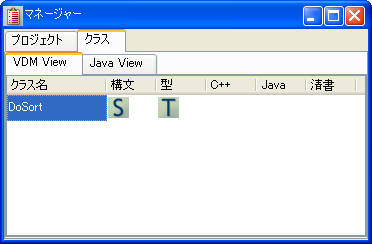
\includegraphics{toolbox}}
\caption{構文および型チェック後の管理画面}\label{fig:toolbox}
\end{center}
\end{figure}

ここで、 \raisebox{-1.0mm}{
\includegraphics[width=0.03\textwidth]{java}}
(\guicmd{Javaコード生成}) ボタンをクリックすることで、 {\tt DoSort} クラスに対するコード生成を行うことが出来る。
この操作は複数ファイル/クラスの選択が可能で、その場合はそれらすべてが Javaに変換される。

図~\ref{fig:interpreter} では、{\tt DoSort} クラスに対してどのように Java コードを生成するかを示している。
{\tt  DoSort.java} と呼ばれる Java ファイルがコード生成されていることが示されている。
そのファイルには {\tt DoSort}のJava クラス定義が含まれている。
 {\tt DoSort.java} ファイルが書き込まれるディレクトリは、プロジェクトファイルが置かれている場所となる。
プロジェクトファイルが存在しない場合は、VDM++ Toolbox の起動ディレクトリにファイルは書き込まれる。

\begin{figure}[H]
\begin{center}
\mbox{}
\resizebox{9.2cm}{!}{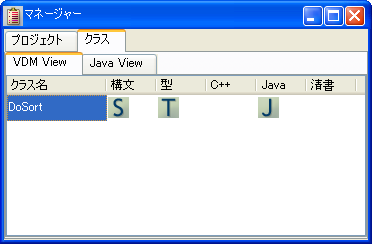
\includegraphics{dosort}}
\caption{{\tt DoSort} クラスをコード生成}\label{fig:interpreter}
\end{center}
\end{figure}

図~\ref{fig:doSortVDM} と図~\ref{fig:doSortJava} は、 {\tt DoSort}クラスに対するVDM++ 仕様の
スケルトンおよび相当するJava生成コードを表す。
生成コードの各部分は、続く章で説明していく。
Appendix \ref{sec:javaDoSort}に、ファイル {\tt DoSort.java} の全体が記載されている。

\begin{figure}[h]
\begin{center}
%\begin{minipage}[t]{2.5in}
%\begin{screen}
\begin{small}
\begin{screen}
\begin{verbatim}  
class DoSort

operations
  public Sort: seq of int ==> seq of int
  Sort(l) ==
    ...

functions

  protected DoSorting: seq of int -> seq of int
  DoSorting(l) ==
    ...

  private InsertSorted: int * seq of int -> seq of int
  InsertSorted(i,l) ==
    ...

end DoSort
\end{verbatim}
\end{screen}
\end{small}
%\end{screen}
%\end{minipage} 
\caption{VDM++ による {\tt DoSort} クラス}\label{fig:doSortVDM}
\end{center}
\end{figure}

\newpage

\begin{figure}[!htb]
\begin{center}
%\begin{minipage}[t]{2.5in}
%\vspace{2cm}
%\begin{screen}
\begin{small}
\begin{screen}
\begin{verbatim}  
public class DoSort {

// ***** VDMTOOLS START Name=vdm_init_DoSort KEEP=NO
  private void vdm_init_DoSort () {}
// ***** VDMTOOLS END Name=vdm_init_DoSort


// ***** VDMTOOLS START Name=DoSort KEEP=NO
  public DoSort () throws CGException {
    ...
  }
// ***** VDMTOOLS END Name=DoSort


// ***** VDMTOOLS START Name=Sort#1|List KEEP=NO
  public List Sort (final List l) throws CGException {
    ...
  }
// ***** VDMTOOLS END Name=Sort#1|List


// ***** VDMTOOLS START Name=DoSorting#1|List KEEP=NO
  protected List DoSorting (final List l) throws CGException {
    ...
  }
// ***** VDMTOOLS END Name=DoSorting#1|List


// ***** VDMTOOLS START Name=InsertSorted#2|Number|List KEEP=NO
  private List InsertSorted (final Number i, final List l)
    throws CGException {
    ...
  }
// ***** VDMTOOLS END Name=InsertSorted#2|Number|List

}
\end{verbatim}
\end{screen}
\end{small}
%\end{screen}
%\end{minipage}
%Java
\caption{生成されたJava {\tt DoSort} クラス\label{fig:doSortJava}}
\end{center}
\end{figure}


 \ToolboxName のコマンドライン版からも、Javaコード生成は可能である。
 \ToolboxName\ は、コマンド {\tt \vdmde}\index{vdmde!starting}を用いることでコマンドラインから始動される。 
Javaコード生成には、 {\tt -j} オプションを用いる。 
クラス{\tt DoSort}のコード生成を行う場合、以下のコマンドを実行する:

\begin{screen}
\begin{verbatim}
vppde -j Sort.vpp
\end{verbatim}
\end{screen}

最初に仕様が構文解析される。
構文エラーが検出されない場合は、仕様に対してPOS型の適格性型のチェックがなされることになる。
もし型エラーが検出されなかったならば、最後に、仕様は複数の Java ファイルに変換される。 
例に挙げている仕様に対しては、{\tt DoSort} クラス定義を含む {\tt DoSort.java} ファイルが生成される。

\begin{description}
  \item[注意] もし、仕様が複数のクラスを含んでいる場合、 \Tcg\ のコマンドライン版を用いると、
              すべてのクラスが同時にコード生成されることになる({\tt -K} オプションでクラス指定が可能)。
\end{description}

%For each \VDM\ class, one Java file is generated.
%This \path+<ClassName>.java+ file contains the definition of the Java class
%corresponding to the \VDM\ class.

\subsection{生成コードとのインターフェース}\label{interfacinggettingstarted}

ここまでで、 \VDM\ 仕様からJava コードを生成ができている。
次に、1個のアプリケーションとしてコンパイルおよび実行するための、
生成された {\tt DoSort} クラスとのインターフェースの記述方法をを示す。

最初に \VDM{}を使ったメインプログラムを示す。

\begin{screen}
\begin{verbatim}
01:  Main() ==
02:    let arr = [23,1,42,31] in  
03:    ( dcl res : seq of int = [],
04:      dos : DoSort := new DoSort();
05:      res = dos.Sort(arr);
06:  )
\end{verbatim}
\end{screen}

上記の \VDM\ 仕様と同機能のJavaのメインプログラムを実装する。
メインプログラムを含むJava ファイルは、
\JL{}パッケージ{\tt jp.vdmtools.VDM}の全クラスをインポートすることから始める。

\begin{screen}
\begin{verbatim}
import jp.vdmtools.VDM.*;
\end{verbatim}
\end{screen}

これにより、完全に修飾された名称を記述することを省略することができる。
\JL{} については、第~\ref{VDMlib}章にさらなる詳細を記述する。
ここでは順を追って、上記のVDM仕様をJavaに変換する。

行 \path+02+ では整数の列を指定する。
Javaに変換すると、以下のコードになる。
\begin{screen}
\begin{verbatim}
List arr = new ArrayList();
arr.add(23);
arr.add(1);
arr.add(42);
arr.add(31);
\end{verbatim}
\end{screen}

{\tt ArrayList}クラスと{\tt List}インターフェースは \texttt{java.util} パッケージに含まれている。
{\tt DoSort}クラスの{\tt Sort}メソッドでは、{\tt List} 型のオブジェクトが入力として要求される。

行 \path+03+ では {\tt seq of int}型の変数 \path+res+ を宣言し、後でソートされた整数列を含めるために用いられる。
これに対応するJava コードは次の通り。

\begin{screen}
\begin{verbatim}
List res = new ArrayList();
\end{verbatim}
\end{screen}

{\tt DoSort}クラスの {\tt Sort} メソッドを呼び出す方法を示そう。
行 \path+04+ では、\path+DoSort+ クラスのインスタンスに対してオブジェクト参照 \path+dos+ を宣言し、行 \path+05+ では、引数としての整数列 \path+arr+ と共に \path+DoSort+ クラスの\path+Sort+ メソッドを呼び出している。
結果は\path+res+に代入される。
Javaに変換すると、以下のコードとなる。

\begin{screen}
\begin{verbatim}
System.out.println("Evaluating Sort("+UTIL.toString(arr)+"):");
DoSort dos = new DoSort();
res = dos.Sort(arr);
System.out.println(UTIL.toString(res));
\end{verbatim}  
\end{screen}

\JL{} の一部である {\tt UTIL.toString} メソッドを用いて、VDM値の文字表現を含む文字列を得る。
このメソッドは、ここでは実行中に結果をログメッセージとして標準出力に出力するために使用されている。

上記の Java コードは、生成されたJavaコード内のメソッドで発生する例外を取り扱うために、
{\tt try} ブロック内に書かれていなければならない。
{\tt try} ブロックには {\tt catch節}が続き、これらの例外を捉えて処理を行う。
生成された Java コードによって起こされる例外はすべて {\tt CGException}クラスのサブクラスであり、
これらもまた \JL{}の一部である。
次のような{\tt catch}文が想定される:

\begin{screen}
\begin{verbatim}
try {
...
}
catch (CGException e){
      System.out.println(e.getMessage());
}
\end{verbatim}  
\end{screen}

前述のメインプログラムは、\path+MainSort.java+ という名のファイルに実装され、
付録の \ref{sec:main}に全体が載せてある。

\subsection{Javaコードのコンパイルと実行}\label{compileandrun}

メインプログラムを手書きすることで、Java コードのコンパイルと実行が可能である。

\cg{} のこの版で生成されたJavaコードは、 Java 開発キット \textbf{1.5}版と相性がよい。

メインプログラムは次でコンパイル可能である:
\begin{screen}
\begin{verbatim}
javac MainSort.java
\end{verbatim}  
\end{screen}

 {\tt CLASSPATH} 環境変数が \JL{}すなわち {\tt VDM.jar} ファイルを含めていることを確認しよう。
 もしUnix Bourne シェル または 互換性のあるシェルを用いているのであれば、これは以下のコマンドで行うことができる:

\begin{screen}
\begin{verbatim}
CLASSPATH=VDM_Java_Library/VDM.jar:$CLASSPATH
export CLASSPATH
\end{verbatim}  
\end{screen}%$

 \JL{} がインストールされたディレクトリ名称を {\tt VDM\_Java\_Library} と置き換えよう。

もし Windowsベースのシステムを使用しているのであれば、 \texttt{CLASSPATH}環境変数は \texttt{autoexec.bat} において、あるいはコントロールパネルのシステムアイコンから、更新できる。
 Windowsに対しては、区切り文字は ``{\tt :}'' ではなく ``{\tt ;}'' を用いなければならないことに注意しよう。

メインプログラム \path+MainSort+ は、これで実行可能である。 
この出力を以下に載せる。
\begin{screen}
\begin{verbatim}
$  java MainSort
Evaluating Sort([23, 1, 42, 31]):
[1, 23, 31, 42]
$
\end{verbatim}
\end{screen}

この章では、どのように \tcg を使用するかについて、簡単な導入を示した。 
以下の章ではもう少し詳細に \tcg\ の様々な局面を記述する。
以降は、生成コード部分の提示は常に、論点に関連する部分のみのテキスト提示とするので注意しよう。

\newpage
\section{コードジェネレータ − 詳細編}
\label{advancedissues}

第~\ref{invoking}章では \tcg{} への簡単な導入を示した。
この章は、以下に続く質問への答えを与えることになる:

\begin{itemize}
\item VDM++仕様からJavaコードを生成するときに、どのようなオプションを使用できるか? (第~\ref{options}章) 
\item 仕様が陰関数/操作または仮関数/操作を含む場合には、何が行えるか? (第~\ref{implicit}章) 
\item 生成されたJavaコードを手書きコードと置き換える可能性は? (第~\ref{substituting}章) 
\item  \VDM\ 仕様がコンパイル可能な正しいJavaコードに変換されるために満たすべき要件は何か?
(第~\ref{sec:unsupported}章) 
\end{itemize}

\subsection{Javaコードジェネレータのオプション}
\label{options}

VDM++ 仕様からJavaコードを生成するとき、生成コードに影響を与える1つ以上の次のオプションを選択することができる。
利用可能なオプションを見るために、図~\ref{fig:optionsmenu}に示すように、
プロジェクトオプションメニューから \textit{Javaコード生成} タブを選択しよう。

\begin{figure}[H]
\begin{center}
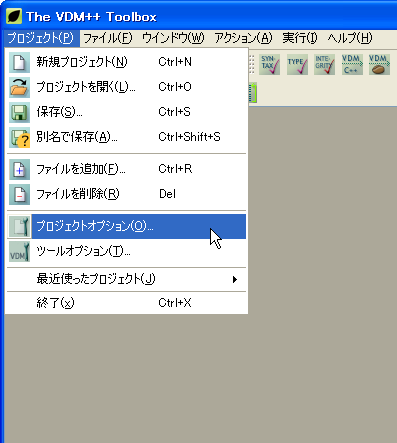
\includegraphics[width=.8\textwidth]{optionsmenu}
\caption{Java コードジェネレータのオプションの選択}\label{fig:optionsmenu}
\end{center}
\end{figure}

図~\ref{fig:options}に示されるように、 \tcg\ において様々なオプションが利用可能である。
\begin{figure}
\begin{center}
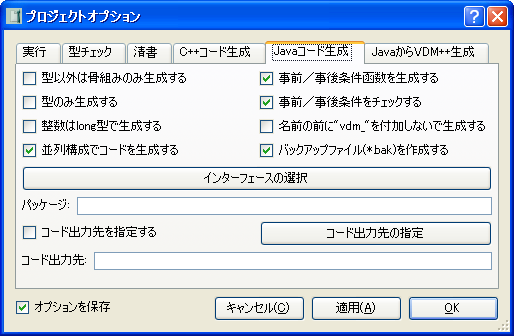
\includegraphics[width=.8\textwidth]{options}
\caption{Java コード生成のためのオプション}\label{fig:options}
\end{center}
\end{figure}
これら各オプションの説明は以下に記述している。

これらオプションのいくつかは、 \tcg のコマンドライン版でも利用可能であることに注意しよう。
以下の各オプション名称の後の括弧内に、対応するフラグを提示している。
デフォルトの動作もまた、デフォルトで与えられたオプションで指定された動作が用いられないという
意味の ``off'' や、動作が用いられるという意味の ``on'' に記載されている。

\begin{description}
\item [型以外は骨組みのみ生成する ({\tt -s})] 
  スケルトンクラスを生成するために、このオプションを指定する。
スケルトンクラスはすべての型、値、インスタンス変数定義を含むが、空の関数や操作の定義は含まないクラスである。 \\
デフォルト: \textbf{off}
%\item [Code generate small types] 
%  The default behaviour of the Code Generator is to
%  generate code with ``big'' types, i.e.\ the wrapper classes {\tt
%  Integer}, {\tt Double}, {\tt Boolean} and {\tt Character} are used
%  in the generated code. Specify the {\tt -m} option in order to
%  generate code using the ``small'' types   {\tt int}, {\tt double},
%  {\tt boolean} and {\tt char}. Note, that ``small'' types are only
%  used in type definitions and method headers. Therfore, this option
%  implies the {\tt -s} option, because otherwise the generated code
%  would not be compilable. It is not possible to insert primitive
%  data types in compound data types such as sets and sequences. %{\tt -m}
\item [型のみ生成する ({\tt -u})] 
  VDM++ 型定義に対してJavaコードを生成したいというだけのとき、このオプションを指定する (つまり 関数、操作、インスタンス変数、値、は生成されない)。 \\
デフォルト: \textbf{off}.%
\item [整数はlong型でコードを生成する ({\tt -L})]
  このオプションを使用することで、VDM++ 整数値と変数をJavaの\texttt{Integer}ではなく \texttt{Long}として生成が可能である。 \\
デフォルト: \textbf{off}
\item [並列構成でコードを生成する ({\tt -e})]
  このオプションは、コードジェネレータが並列支援を含めるコード生成を行うために用いられる。
この詳細は第~\ref{concmain}章を参照のこと。 \\
デフォルト: \textbf{on}
\item [事前/事後条件函数を生成する ({\tt -k})] 
事前事後条件に対するJavaメソッドやそれらの不変条件をコード生成するために、 このオプションを指定する。 \\
デフォルト: \textbf{on}
\item [事前/事後条件をチェックする ({\tt -P})] 
 このオプションを、関数の事前事後条件のインラインチェック生成のために指定する。
チェックが失敗した場合に例外を発生する。
この意味は、事前事後条件としての前述のオプションが、コンパイル可能なコードのために生成されるべきであることを含めている。 \\
デフォルト: \textbf{off}
\item [名前の前に``vdm\_''を付加しないで生成する] 
 このオプションは、VDM++のクラス名がJDKのクラス名と同じ場合に、``vdm\_''を付加せずに生成するために用いられる。 \\
デフォルト: \textbf{off}
\item [バックアップファイル(*.bak)を作成する] 
 このオプションは、以前に生成したjavaファイルを保存するために用いられる。 \\
デフォルト: \textbf{on}
\item [インターフェースの選択 (\texttt{-U classname[{,classname}]})]
  Javaインターフェースとして生成されるべきクラスを選択する。詳細は第~\ref{sec:interfaces}章を参照。
\item [パッケージ ({\tt -z}) \textit{packagename}] 
  コードジェネレータの既定の動作は、ディレクトリ内に生成されたJavaファイルを書き出すことであり、このディレクトリとはプロジェクトファイルが置かれている場所か、あるいはプロジェクトファイルが存在しない場合は \ToolboxName\ がスタートした場所である。
ファイルは名称のない既定パッケージの一部である。 
生成されたJavaクラスを含むはずの指定パッケージを生成するために、このオプションを指定する。
コードジェネレータは、生成ファイルを含めるため与えられたパッケージ名称を使った新しいディレクトリを作成し、生成ファイルには適切な  \texttt{package} 文が含まれることになる。%{\tt -z package\_name}
\item [コード出力先の指定]
生成されるJavaファイルは、プロジェクト名が指定されている場合、プロジェクトファイルと同じディレクトリに生成される。
他の場所に生成したい場合にこのオプションを使用する。\\
\end{description}

コマンドラインから \ToolboxName\ をスタートさせる場合、以下のコマンドを用いる。  

\begin{screen}
\begin{verbatim}
vppde -j [options] specfile(s)
\end{verbatim}
\end{screen}


\subsection{陰関数/操作および仮関数/操作の実装}\label{implicit}

陰関数/操作および仮関数/操作(``{\tt is not yet specified}''で指定されたもの) が、
\tcg{}によっても同じ方法で取り扱える。 
仮操作定義を含む以下の VDM++ クラス定義を見よう。

\begin{screen}
\begin{verbatim}
class A
operations
op:() ==> int
op() == is not yet specified;
end A
\end{verbatim}
\end{screen}

このクラスは以下のように生成されることになる。

\begin{screen}
\begin{verbatim}
public class A {
  protected external_A child = new external_A(this);
  private Integer op () throws CGException{
    return child.impl_op();
  }
};
\end{verbatim}
\end{screen}

上述のコードから見てとれるように、クラス \texttt{A} は型{\tt external\_A}の
{\tt protected} なインスタンス変数 {\tt child} を保有している。
これは、陰関数/操作または仮(``{\tt is not yet specified}''で指定された)関数/操作が記述されている
すべてのクラスに当てはまる。
クラスがこれらの定義をいくつか含んでいるとしても、その外部クラスは1つのインスタンスしか存在しないはずである。

\path+op+ メソッドは、このインスタンスの \path+impl_op+ という名のメソッドを呼び出すことになる
\footnote{{\tt impl} は ``Javaで実装されるべき''ことを表す。}。 \path+impl_op+ メソッドの結果は
\path+op+ メソッドの結果として返される。

したがってクラス {\tt external\_A}にメソッド\path+impl_op+ を実装することは、ユーザーの責任である。
メソッド \path+impl_op+の入出力パラメータは、メソッド \path+op+のそれと同じでなければならない。

もし VDM++ クラスが1つ以上の陰関数/操作または仮関数/操作(``{\tt is not yet specified}''で指定されたもの)を
含むとすれば、すべてのメソッドが\path+external_<CLASSNAME>+に実装されていなければならない。

ユーザーが外部クラスファイルを実装するのを容易とするために、
\tcg\ はこれに対する \texttt{external\_A.java} ファイルを生成する。
このファイルの支援で、生成された Java コードはコンパイル可能となる。
しかしながら、仮関数が呼ばれた場合は、実行時エラーが起きることになる。
{\tt external\_A}クラスを含む{\tt external\_A.java} ファイルを、以下に示す。

\begin{screen}
\begin{verbatim}
public class external_A {
  A parent = null;
  public external_A (A parentA) {
    parent = parentA;
  }
  public Integer impl_op () throws CGException{
    UTIL.RunTime("Preliminary Operation op has been called");
    return new Integer(0);
  }
};
\end{verbatim}
\end{screen}

{\tt external\_A} クラスを実装する最も簡単な方法は、テンプレートクラスを修正することだ。
つまり、ユーザーは次のコード部分を、生成コードをユーザ独自のコードで置き換えるというありふれた方法で、
置き換えを行う必要がある。

\begin{screen}
\begin{verbatim}
UTIL.RunTime("Preliminary Operation op has been called");
return new Integer(0);
\end{verbatim}
\end{screen}

(詳細は第~\ref{substituting} 章を参照)


%Once the user has tailored the {\tt external\_<ClassName>.java} file,
%it has to be insured, that a new code generation does not overwrite
%it with a new file. Therefore, when an {\tt
%external\_<ClassName>.java} already exists, an {\tt
%external\_<ClassName>.java.default} file is generated instead. 

注意したいのは、外部クラスに対して生成されたコンストラクタが、入力パラメータとしてクラス
{\tt A} のインスタンスを取り入れ変数 {\tt parent}に代入することである。
この方法で、仮操作定義の実装はクラス {\tt A}のpublicな属性や操作にアクセス可能である。
クラスの内部状態に作用することが許されないため、仮関数に対応するJavaメソッドが
このコンストラクタを用いることになる。
しかしそれらはある操作を呼び出すことで、間接的に内部状態への作用が可能となる。

陰関数/操作は、 ``{\tt is not yet specified}''節を含む
仮関数/操作の仕様と同じ方法で取り扱われる。

注意したいのは、外部クラスが陰関数/操作と仮関数/操作の両方を含むことが可能であることだ。
生成されたテンプレートにおいて、生成される実行時エラーメッセージの違いで区別可能である。

\begin{screen}
\begin{verbatim}
UTIL.RunTime("Preliminary Operation op has been called");
\end{verbatim}
\end{screen}

これは {\tt op} という名の仮操作定義に対するものであり、

\begin{screen}
\begin{verbatim}
UTIL.RunTime("Implicit Function f has been called");
\end{verbatim}
\end{screen}

これは {\tt f}という名の陰関数定義に対するものある。

\subsection{抽象クラスの生成}

VDM++ クラスは、仮関数あるいは操作の定義を含むか、あるいは抽象クラスのサブクラスであり、
継承している抽象関数・操作の実装を提供しない場合に、抽象クラスとなる。

一方で、Java においても抽象クラスの基本概念を提供している。
したがって、Java コードを生成するときに、抽象クラスと識別される VDM++ クラスは、
抽象Javaクラスとして生成されることになる。
例えば、 以下のVDM++ クラス \texttt{A}、\texttt{B} 、\texttt{C} を考察してみよう。

\begin{screen}
\begin{verbatim}
class A

instance variables
  protected m : nat := 1

operations
  public op : nat ==> nat
  op(n) == is subclass responsibility;

functions
  public f : int -> int
  f(i) == is subclass responsibility

end A

class B is subclass of A

operations
  public op : nat ==> nat
  op(n) ==
    return m + n

end B

class C is subclass of B

functions
  public f : int -> int
  f(i) == i + 1

end C
\end{verbatim}
\end{screen}

クラス \texttt{A} は仮関数・操作を含むので、抽象クラスである。
したがって次のようなコード生成がなされる。

\begin{screen}
\begin{verbatim}
public abstract class A {
 
  protected Integer m = null;
  public abstract Integer op (final Integer n) throws CGException;
  public abstract Integer f (final Integer i) throws CGException;
 
} 
\end{verbatim}
\end{screen}
クラス \texttt{B} は抽象クラス \texttt{A}を継承し、関数 \texttt{f}の実装を提供していない。
したがって抽象でもある。

\begin{screen}
\begin{verbatim}
public abstract class B extends A {

  public Integer op (final Integer n) throws CGException {
    return new Integer(m.intValue() + n.intValue());
  }
}
\end{verbatim}
\end{screen}

最後は、クラス \texttt{C} は \texttt{B} から継承し、 \texttt{f}の実装を提供するためにある。
したがって通常のクラスである。
\begin{screen}
\begin{verbatim}
public class C extends B {
 
  public Integer f (final Integer i) throws CGException{
    return new Integer(i.intValue() + new Integer(1).intValue());
  }
} 
\end{verbatim}
\end{screen}


\subsection{生成された Java コード部分の置き換え}\label{substituting}

標準的な応用として、生成コードに対し、例えば外部ライブラリや手書きコードといった
他コードと相互作用を行う必要が生じてくるだろう。
このような相互作用を手助けするため、生成コードの修正が可能で、しかも \tcg\ が
再実行されてもそれらの修正が上書きされない方法がある。

これは、 \textit{KEEPタグ}の使用を通して実現される。
これらは生成されたJavaコードにおいてはコメントであるが、 そのコードが
上書されるべきか否かを \tcg\ が決定するときに用いるものである。

例えば以下の例題を考えよう。
\begin{screen}
\begin{verbatim}
class Date

types
  public Day = <Mon> | <Tue> | <Wed> | <Thu> | <Fri> | <Sat> | <Sun>;
  public Month = <Jan> | <Feb> | <Mar> | <Apr> | <May> | <Jun> 
        | <Jul> | <Aug> | <Sep> | <Oct> | <Nov> | <Dec>;
  public Year = nat

instance variables
  d : Day;
  m : Month;
  y : Year

operations

  public SetDate : Day * Month * Year ==> ()
  SetDate(nd,nm,ny) ==
  ( d := nd;
    m := nm;
    y := ny );

  public today : () ==> Date
  today() ==
    return new Date()
end Date
\end{verbatim}
\end{screen}
 VDM++ も \ToolboxName\ も時間の基本概念を持たないため、\texttt{today}に完璧な仕様を与えることはできない。 
生成コードで \texttt{today} は次のようになる。
\begin{screen}
\begin{verbatim}
// ***** VDMTOOLS START Name=today KEEP=NO
  public Date today () throws CGException{
    return (Date) new Date();
  }
// ***** VDMTOOLS END Name=today
\end{verbatim}
\end{screen}
関数定義の上下のコメントは、この関数に対するKEEPタグに相当する。
KEEPタグでは以下の情報が得られる。
\begin{itemize}
\item タグが適用される実体の名称 (実体を構成するものは次で述べられる)。
 テキスト\texttt{Name=}の直後に置かれる。
\item この実体が保存されるべきか上書きされるべきかを示すフラグ。 
 \texttt{KEEP=}の後にテキストで与えられる。
もし\texttt{NO}ならば実体は上書きされ、 \texttt{YES}ならば保存される。
ファイル生成時のデフォルトは \texttt{NO}である。
\end{itemize}
現在の日付を返すように、この関数を修正したいと仮定する。
これは、Java 開発キット(JDK)の一部として提供されている \texttt{Calendar} クラスを用いて可能である。
\begin{screen}
\begin{verbatim}
// ***** VDMTOOLS START Name=today KEEP=YES
  public Date today () throws CGException{
    Calendar c = Calendar.getInstance();
    Date result = new Date();
    Object td = new Object(), tm = new Object();
    switch (c.get(Calendar.DAY_OF_WEEK)){
    case Calendar.MONDAY:
        td = new quotes.Mon();
        break;
    ...
    }
    switch (c.get(Calendar.MONTH)) {
    case Calendar.JANUARY:
        tm = new quotes.Jan();
        break;
    ...
    }
    result.SetDate(td, tm, c.get(Calendar.YEAR));
    return result;
  }
// ***** VDMTOOLS END Name=today
\end{verbatim}
\end{screen}
最初にKEEPタグが \texttt{YES}に変化していることに注意しよう。
これは変更が保存されることを保証している。
関数本体はしたがって通常のJava コードであり、任意の外部クラスで用いることができる。

現存の実体の変更に加えて、 Java ファイルに新しい実体の追加ができる。 
既定の\texttt{toString} メソッド ( \texttt{java.lang.Object}から継承)を
日付に適用したものに置き換えたいと仮定しよう。
以下をクラス定義に追加できるだろう。
\begin{screen}
\begin{verbatim}
// ***** VDMTOOLS START Name=toString KEEP=YES
  public String toString() {
      return d.toString() + m.toString() + y.toString();
  }
// ***** VDMTOOLS END Name=toString
\end{verbatim}
\end{screen}

\subsubsection{実体}

KEEPタグを用いて保存できた生成 Java ファイルにおいて、実体は1つの領域である。
これは以下の1つとなる可能性がある。

\begin{itemize}
\item トップレベルのクラスメンバー変数
\item トップレベルのクラスメソッド(コンストラクタを含む)
\item インナークラス
\item インポート宣言の集まり
\item パッケージ宣言
\item ヘッダーコメント(ファイルの先頭領域に、例えばバージョン管理情報といったコメントを置くことができる)
\end{itemize}
KEEPタグは、interfaceとして生成されたクラスと共に用いられることもあることは注意しよう
(第~\ref{sec:interfaces}章参照)。
この場合も同じ規則が適用され、クラスの代わりにinterfaceが読み込まれる。

事前に定義された3つのタグ名称、ヘッダーコメントのための\texttt{HeaderComment}・
パッケージ宣言のための\texttt{package}・インポート宣言のための \texttt{imports} 、は生成されたファイル中でよく現れる。

\subsubsection{KEEPタグのための規則}

KEEPタグを使用するときは以下の規則に従わなくてはならない。 

\begin{itemize}
\item 各タグ名称は唯一のものでなければならない
\item タグは同一レベルでなければならない、つまりタグのネストは不可能である
\item クラス定義の外部のみで現れる可能性のあるタグは、\texttt{HeaderComment}・ \texttt{package} ・ \texttt{imports}である
\item 付加された実体はクラス定義の \textbf{内部に} 、それも先頭部分に現れなければならない
(例えばある関数がインナークラスに追加された場合、インナークラス全体が \texttt{YES} とタグづけされなければならない)
\item KEEPタグの構文では、case文と空白は細心の注意を払うべきであり、正確に後ろを続けていく必要がある
\end{itemize}

これらの規則に従わないとき、コードは上書きされてしまう可能性がある。
しかしながら、オプション設定で、元のファイルをバックアップするよう設定しておけば、必ずしもこれが致命的となることはない。


\subsection{interfaceの生成}\label{sec:interfaces}

\Tcg\ は Javaのinterface \cite{Gosling&00}の生成を可能としている。
 \VDM\ クラスは以下の条件に適応する場合は、interfaceとして生成される可能性がある。

\begin{itemize}
\item このクラスで定義された関数と操作のすべてが、本体 \texttt{is subclass responsibility}である
\item インスタンス変数を含まないクラスが、このクラス中に定義されている
\item このクラスで定義されたすべての型が、publicである
\item このクラスで定義されたすべての値は、直接の定義が可能である (直接定義される値の意味の説明は第~\ref{values}章を参照)
\item このクラスのすべてのスーパークラスはinterfaceとして生成可能である
\end{itemize}

例えば、図~\ref{fig:interfacesex}の例題を考えてみよう。
\begin{figure}
\begin{screen}
\verbatiminput{manexamples/interfaces.vpp}
\end{screen}
\caption{インターフェース例題}\label{fig:interfacesex}
\end{figure}
クラス \texttt{A} は明らかにinterfaceとして生成されるための要件を満たす。
なぜなら、直接定義された値をもち、その関数と操作すべてが \texttt{is subclass responsibility}だからである。
クラス \texttt{B} もまたinterfaceとして生成可能だ。なぜなら抽象関数1つだけが与えられ、
interfaceとして生成が可能なクラスを継承しているからである。
しかしクラス \texttt{C}はinterfaceとして生成はできない。
なぜなら抽象でない関数の宣言を行っているからである。

どのクラスをinterfaceとして生成するべきかの選択には、
プロジェクトオプションダイアログ(第~\ref{options}章に記述されている) 
の \texttt{インターフェースの選択} ボタンをクリックしよう。 
図~\ref{fig:interfaces1}で示すように、新しいダイアログボックスが開く。 

\begin{figure}
\begin{center}
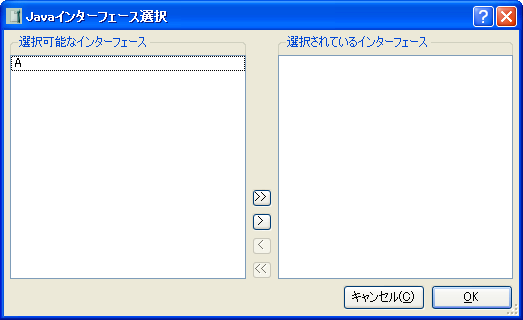
\includegraphics[width=.8\textwidth]{interfaces1}
\end{center}
\caption{最初のインターフェース選択ダイアログ}\label{fig:interfaces1}
\end{figure}

最初は、interface -\texttt{A}としては唯1つクラスが生成される可能性がある。
これが選択されると ( \textit{追加}ボタンをクリックすることにより)、
図~\ref{fig:interfaces2}に示されるようにダイアログは更新される。

\begin{figure}
\begin{center}
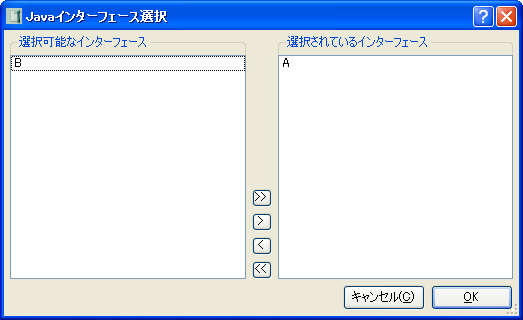
\includegraphics[width=.8\textwidth]{interfaces2}
\end{center}
\caption{更新されたインターフェース選択ダイアログ}\label{fig:interfaces2}
\end{figure}

ここで可能なinterfaceの一覧に \texttt{B} が現れていることに注目しよう。 
もしこのスーパークラス - \texttt{A} - がinterfaceであるならば、
これはinterfaceとして生成されることのみ可能となるためである。
選択interfaceの一覧から \texttt{A} が取り除かれたら、\texttt{B}は自動的に一覧から取り除かれる。
その時点でもはやinterfaceの基準を満たさないからである。

インターフェースとして生成されるべきクラスが選択されると、コード生成は通常通りに開始する。
\texttt{A}に対して以下のコードが生成されるはずである。

\begin{screen}
\begin{verbatim}
public interface A {
 
// ***** VDMTOOLS START Name=v KEEP=NO
  public static final Number v = new Integer(1);
// ***** VDMTOOLS END Name=v


// ***** VDMTOOLS START Name=op#1|Number KEEP=NO
  abstract public Number op (final Number n) throws CGException ;
// ***** VDMTOOLS END Name=op#1|Number


// ***** VDMTOOLS START Name=f#1|Number KEEP=NO
  abstract public Number f (final Number n) throws CGException ;
// ***** VDMTOOLS END Name=f#1|Number

} 
\end{verbatim}
\end{screen}

Toolboxのコマンドライン版を用いてもまたinterfaceの選択は可能であり、この場合 \texttt{-U} オプションを用いる。
\begin{screen}
\begin{alltt}
vppde -j -U \textit{class\{,class\}} specfiles
\end{alltt}
\end{screen}

もしクラスが上記のインターフェース基準を満足させないとする場合、以下のエラーメッセージが表示されるだろう。

\begin{screen}
\begin{alltt}
Can not generate class \textit{class} as an interface - ignored
\end{alltt}
\end{screen}



\subsection{制限}\label{sec:unsupported}

すべての \VDM\ 仕様でJavaコード生成が可能というわけではない。 
コンパイル可能で正しいJavaコードに変換されるために、 \VDM\ 仕様はある要件を満たす必要がある。
これらの制限は主に2つの理由が原因で引き起こされる: 

\begin{description}
\item[用いられる変換アルゴリズムの制限] \VDM\ および Java は2つの異なる言語であること。 
数少ない例として、 \VDM\ 構成要素の何らかの変換が正しくないJavaコードを導く可能性がある。 
このことから引き起こされる制限は、第~\ref{lim1}章に並べている。
これらの要件を満たさない\VDM\ 仕様は、コンパイル可能でない誤ったJavaコードに変換される可能性がある。
Javaへ変換できない \VDM\ の機能にぶつかると、 \Tcg\ は警告/エラーメッセージを表示する。
\item[変換の範囲制限] コードジェネレータはすべての構成要素をサポートしているわけではない。 
第~\ref{lim2}章では、 \tcg{}でサポートされない \VDM\ 構成要素をまとめている。
これらの構成要素はコンパイルできないJavaコードではないが、これらに対して生成されたコードを実行すると実行時エラーとなる。
\Tcg\ はサポートされていない構成要素に出会えば必ず、警告を与えることになる。
\end{description}

Java と VDM++ の意味論においては、プライベートメソッドが、動的ディスパッチに関してどう扱われるかが異なることに注意しよう。 
以下の例題を考える。

\begin{minipage}{.50\textwidth}
\begin{screen}
\begin{verbatim}
class C
operations
public op1 : () ==> seq of char
op1() == op2();

private op2 : () ==> seq of char
op2() == return "C`op2"
end C
\end{verbatim}
\end{screen}
\end{minipage}
\begin{minipage}{.50\textwidth}
\begin{screen}
\begin{verbatim}
class D is subclass of C
operations
public op3 : () ==> seq of char
op3() == op1();

private op2 : () ==> seq of char
op2() == return "D`op2"
end D
\end{verbatim}
\end{screen}
\end{minipage}

Javaにおいて、式 \texttt{new D().op3()} は\texttt{C`op2}という結果となる。
一方、\VDM\ においては、同じ式が \texttt{"D`op2"}となる。

\subsubsection{言語の違いに起因する \VDM\ 仕様の要件}
\label{lim1}

\VDM\ 仕様は、 {\em コンパイル可能} で {\em 正しい} Java コードを生成するために、以下の要件を満たさなければならない。

\begin{itemize}
\item ``{\em 型情報不明}''という型チェッカー警告は取り除かれるべきである。
これは、生成コードにエラーが含まれる可能性があるからである。
もしVDM 構成要素の型情報がない場合、\Tcg\ は正しいJava型の生成ができない。

\item クラス、インスタンス変数、型、値、関数、操作に同じ名称を付けてはならない。
%さらには、名称の再宣言は避けるべきである。
%この意味は、例えば以下の \VDM\ 仕様は変数名称 {\tt a} が再宣言されているため、
%コンパイル不可能な結果となるだろう、ということである:
%
%\begin{screen}
%\begin{small}
%\begin{verbatim}
%f : int | (int * int) ==> bool
%f(a) ==
%  cases a:
%    2 -> return true,
%    mk_(a,b) ->  return false,
%    others -> let a = 1 in return true
%  end;
%\end{verbatim}
%\end{small}
%\end{screen}

\item 抽象の操作/関数は、それらを実装する操作/関数と同じ型をもつ必要がある。
以下の例題を考えよう。
\begin{screen}
\begin{small}
\begin{verbatim}
class A
operations
  m: nat ==> nat
  m(n) == is not yet specified;
end A

class B is subclass of A
operations
  m: nat ==> nat
  m(n) = return n+n;
end B
\end{verbatim}
\end{small}
\end{screen}
もし\texttt{B`m} の型が\texttt{A`m}の型と正確に一致しない場合、
\texttt{A`m} は \texttt{B}においても抽象操作であり、したがって \texttt{B}は抽象クラスということになる。

\item 多重継承には一定の制限がある。 
これに含まれるクラスは第~\ref{sec:interfaces}章に記載された条件を満たしている必要がある。

\item case文のすべての場合分けがreturn文が含まれる場合、
case文は {\tt others} をもたなくてはならない。
そうでない場合には、Java コンパイラが生成されたJavaコードをコンパイルすると、
``{\em Return required}'' エラーを生成する。

\item 不要なコードは避けるべきである。 
以下の例題を考えよう。

\begin{screen}
\begin{small}
\begin{verbatim}
operations
  m : nat ==> nat
  m(n) ==
    (return n;
     a:= 4;
    );
\end{verbatim}
\end{small}
\end{screen}

文 {\tt a:= 4;} は決して実行されることはなく、生成されたJavaコードをコンパイルすると、
``{\em Statement not reached}'' エラーが生じる。

\item スーパークラスにおける操作呼出しを、クラス名で修飾した場合、生成コードは誤ったものとなる可能性がある。
以下の例題を見よう。

\begin{screen}
\begin{small}
\begin{verbatim}
class A

operations
  public SetVal : nat ==> ()
  SetVal(n) == ...;

end A

class B is subclass of A

operations
  public SetVal : nat ==> ()
  SetVal(n) == ...

end B

class C is subclass of B

operations
  public Test : () ==> ()
  Test() ==
    ( self.SetVal(1);
      self.B`SetVal(1);
      self.A`SetVal(2)
    )

end C

class D

instance variables
  b : B := new B()

operations
  public Test: () ==> ()
  Test() ==
    (b.SetVal(1);
     b.B`SetVal(5);
     b.A`SetVal(2)
    )

end D
\end{verbatim}
\end{small}
\end{screen}

まずはクラス {\tt C}から見よう: 
文 {\tt self.SetVal(1)}はクラス {\tt C}における {\tt SetVal} 操作を呼び出し、
Javaにおいて {\tt this.SetVal(1)} としてコード生成されることになる。
文 {\tt self.B`SetVal(1)}はクラス {\tt B}における{\tt SetVal}操作を呼び出し、
Javaにおいて {\tt super.SetVal(1)} としてコード生成されることになる。
Java では、クラス{\tt A}の {\tt SetVal()} メソッド呼び出しは不可能である。
文 {\tt self.A`SetVal(2)} は {\tt super.SetVal(2)}としてコード生成されるだろう。
クラス {\tt B}に {\tt SetVal} 操作がなかったなら、これは正しくなるはずである。
しかし上記の場合、これは VDM++ 仕様に適合しない。
2つの操作呼び出し {\tt self.B`SetVal(1)} と {\tt self.A`SetVal(2)}に対して、
コードジェネレータは、警告 ``{\em Quoted method call はスーパークラスの呼び出しとしてコード生成されます}''を生成する。
これにより、正しいメソッドが呼び出されるかどうかの確認を行わねばならないことがわかる。
  
次にクラス {\tt D}を見よう: 
文 {\tt b.SetVal(1)} はクラス {\tt B}の {\tt SetVal} 操作を呼び出し、
Javaで {\tt b.SetVal(1)} としてコード生成されることになる。
Javaではオーバーライドしているクラスの外部からオーバーライドされたメソッドを起動することはできない。
したがってクラス {\tt A}で {\tt SetVal}メソッドを呼び出す方法はない。
クラス {\tt D}で引用された操作呼び出しは、すべて {\tt b.SetVal(1)}としてコード生成される。 
この場合、コード生成は、警告 ``{\em Quoted method call が削除されています}'' 生成し、ユーザに通知する。

\item Javaにおける整数型および倍精度浮動小数点型の最大 (最小)値が、 \VDM{}のそれぞれの値より小さい(大きい)。
Javaでは有効でない値があると、生成されたJavaコードの実行時にエラーが発生する。
\end{itemize}

\subsubsection{サポートされていない構成要素}
\label{lim2}

 \tcg\ では、以下の \VDM\ 構成要素はサポートされていない。

\begin{itemize}

%% Is not part of the language manual any longer!
%\item The Real-time part of \VDM{}. 
\item 式

  \begin{itemize}
  \item ラムダ式
  \item 関数に対する合成、繰り返し、同等
  \item 型変数を含む型判定式
#ifdef VICEMAN
  \item time式
#endif VICEMAN
  \item 高次関数
  \item ローカル関数定義
  \item 関数型インスタンス化式 \\ しかし、以下の例題の中にあるように、コードジェネレータが適用式と組み合わさることで関数型インスタンス化式をサポートする

\begin{screen}
\begin{verbatim}
Test:() -> set of int
Test() ==
  ElemToSet[int](-1);

ElemToSet[@elem]: @elem +> set of @elem
ElemToSet(e) ==
  {e}
\end{verbatim}
\end{screen}

  \end{itemize}

\item 文
  \begin{itemize}
  \item 仕様記述文
#ifdef VDMSL
  \item call文内の `{\sf using}'
#endif VDMSL
%#ifdef VDMPP
%  \item startlist文
%#endif VDMPP
#ifdef VICEMAN
  \item duration文とcycles文は無視される
#endif VICEMAN
  \end{itemize}

\item 型束縛 (\langmancite 参照)ただし次の中

  \begin{itemize}
  \item Let-be-st 式/文
  \item 列、集合、写像の包括式
  \item Iota式 と修飾式
  \end{itemize}

例題として、以下の式が\tcg によりサポートされている。

\begin{screen}
\begin{verbatim}
let x in set numbers in x
\end{verbatim}
\end{screen}

一方で以下はサポートされていない (型束縛 \verb+x : nat+に起因する)。

\begin{screen}
\begin{verbatim}
let x: nat in x
\end{verbatim}
\end{screen}

\item パターン(簡単なものはコード生成可能)

  \begin{itemize}
  \item 集合合併パターン。
  \item 列連結パターン。
  \item 写像併合パターン。
  \end{itemize}

#ifdef VDMSL
\item Local Function Definitions.

\item Higher order function definitions.
  
\item Function Values. 

\item Parameterized modules.
#endif VDMSL
\end{itemize}

#ifdef VICEMAN
CPUとBUSesへのシステム仕様と対応する展開は無視されます。
Javaコードがそのようなシステム記述から生成されると、生成コードは、役に立たなく、コンパイルできないでしょう。
同様に、操作定義の \keyw{async} キーワードは無視されます。
#endif VICEMAN

\Tcg\ はこれらの構成要素を含む仕様に対してコンパイル可能なコードを生成できるが、
サポートされていない構成要素を含む分岐が実行された場合は、コードの実行は実行時エラーという結果となる。
以下の関数定義を考えよう。

\begin{screen}
\begin{verbatim}
f: nat -> nat
f(x) ==
  if x <> 2 then
    x
  else
    iota x : nat & x ** 2 = 4
\end{verbatim}
\end{screen}

\path+f+ に対して生成されたコードは、コンパイルされることになる。 
しかし \path+f+ に相当するコンパイルされた Java コードは、  \path+f+ に値2が適用されれば、
iota式の型束縛はサポートされず実行時エラーという結果に終わるだろう。 

注意したいのは、 \Tcg\ はサポートされていない構成要素に出会った場合は必ず警告を与えるはずだということである。
上記の関数{\tt f} に対するコード生成では、図~\ref{fig:cg_error}で示される、
{\em Error} ウィンドウが表示される。

\begin{figure}[H]
\begin{center}
\mbox{}
\resizebox{9.2cm}{!}{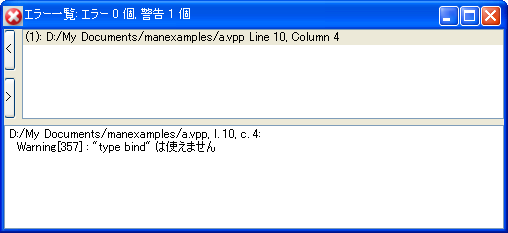
\includegraphics{warning}}
\caption{コードジェネレータにより生成された警告}\label{fig:cg_error}
\end{center}
\end{figure}

\newpage
\section{\VDM\ 仕様のコード生成}
\label{sec:relation}

この章では、 \VDM\ 構成要素がコード生成される方法を詳細に記述していく。
この記述は、\tcg\ を専門的に利用しようとする場合には集中して学習すべき内容である。
始めは \JL{}への導入を行うが、これが \VDM\ 仕様コード生成の基礎を形成する。
その後、上記で述べた \VDM\ 構成要素1つ1つに対して生成されるコードを述べていく。

\subsection{VDM Java ライブラリ}
\label{VDMlib}

生成コードのデータ改編は、 \JL{}に基づき、パッケージ {\tt jp.vdmtools.VDM}に実装されている。
ここでは、このライブラリについて簡単に紹介する。
詳細は、 {\em javadoc} プログラムにより生成されたHTML文書で説明されている。
このライブラリについて詳しく理解したければ、その文書を読むべきである。
 {\em javadoc} プログラムを使用した HTML 文書生成方法についての記述は、付録~\ref{install}を参照のこと。 

 \JL{} は以下の\VDM\ データ型の実装を提供する。

\begin{itemize} 
%\item Sequence Type
%\item Set Type
%\item Map Type
%\item Quote Type
%\item Token Type
%\item Product/Tuple Type
\item 積型/組型
%\item Optional Type
%\item Record Type
\item レコード型
\end{itemize}

これらの型のそれぞれに対して、1つのクラスが、相当するVDM++ 型と同じパブリックメソッドを提供しながら実装されてくる。
これらクラスは Java 言語により提供されたクラスの先頭に実装される。

\VDM\ データ型で上記で並べていないもの(基本データ型、集合型、列型、写像型、オプション型、オブジェクト参照型)は、
Java言語自身の一部であるクラス/構成要素 かあるいはJava開発キット(JDK)の一部配布により表現される。

上記に挙げた \VDM\ データ型の実装の提供に加えて、 \JL{} はさらに2つのクラスを提供する。

\begin{description} 
\item[Utilクラス] このクラスは補助メソッドを含むが、これは生成されたコードに用いられ、またユーザーが生成コードとインターフェースをとるときに使用できる。
これらの補助的メソッドのうちもっとも重要なものを以下に並べる。
\begin{description}
\item[clone] VDM 値を (綿密に) 複製する。しかしながら、\VDM\ クラスと基本 \VDM\ データ型は複製できない。
\item[equals] 2つの VDM 値を比較する。
\item[toString] VDM 値の文字表現を含む列を返す。
\item[RunTime] 実行時エラーが起きたときに呼び出される。
\JL{}で定義されている {\tt VDMRunTimeException}を発生させる。
\item[NotSupported] サポートされていない構成要素が実行されたときに呼び出される。
 {\tt NotSupportedConstructException}を発生させるが、これは \JL{}で定義されているものだ。
\end{description}

\begin{description} 
\item[注意] 常に {\tt UTIL}クラスの{\tt clone}、{\tt toString}、{\tt equals}のメソッドを使用しなければならない。
VDM++ データ型に相当するJavaクラスで定義されたメソッドは用いない。
\end{description}

\item[CGExceptionクラスとそのサブクラス]
  
VDM Java ライブラリのエラー操作は、JavaのExceptionハンドリングに基づいている。 
生成されたJavaコードかあるいはライブラリメソッドの1つによりエラーが検出されたとき例外が発生する。
実装済みエラーは、すべて {\tt CGException} のサブクラスであり、
さらに {\tt java.lang.Exception} クラスのサブクラスである。
例外クラスの継承構造を、図~\ref{fig:exceptionclasses}に示す。

\begin{figure}[tbh]
\begin{center}
\mbox{}
\begin{picture}(400,250)
\put(0,0){\framebox(180,50){VDMLibRunTimeException}}
\put(220,0){\framebox(180,50){NotSupportedConstructException}}
\put(110,100){\framebox(180,50){CGException}}
\put(110,200){\framebox(180,50){Exception}}

\put(90,50){\line(0,1){25}}
\put(310,50){\line(0,1){25}}
\put(90,75){\line(1,0){220}}
\put(200,75){\line(0,1){25}}
\put(200,150){\line(0,1){50}}

\end{picture}
\caption{コードジェネレータの例外を取り扱うJavaクラスの継承構造\label{fig:exceptionclasses}}
\end{center}
\end{figure}

例外の様々な種類は2つの型にグループ分けされる。
\begin{description}

\item[VDMRunTimeExceptionクラスのインスタンス] それらはJava生成コードの中で起動される。 
 \VDM\ 仕様の実行中に起きる実行時エラーに相当する。  

\item[NotSupportedConstructExceptionクラスのインスタンス]
 \tcg\ でサポートされていない構成要素が実行されたときに、それらが起こされる。

\end{description}
\end{description}

\subsection{クラスを生成するコード}
\label{sec:classes}

各 \VDM\ クラスに対して、相当する Java クラスが生成される。
各 \VDM\ クラス要素に対して、Javaクラスで相当する項目が \VDM\ 要素と同じアクセス修飾子をもつことになる。

 \VDM\ 仕様のクラスに対して生成されたJavaクラスの構造を、より詳しく見てみよう。

生成された Java クラスは次を含む:

\begin{itemize}
%\item 静的な \textit{比較器}で、Java開発キットのインターフェース\texttt{java.util.Comparator} を実装しているもの。
%これはツリーベースのデータ構造で用いられ、同等の VDM 概念を実装する。
\item \VDM\ データ型を実装するJavaコード(第~\ref{types}章を参照)
\item \VDM\ 値を実装するJavaコード(第~\ref{values}章を参照)
\item \VDM\ インスタンス変数を実装するJavaコード(第~\ref{sec:instvars}章を参照)
\item 静的初期化 (値が初期化されなければならない場合)
\item インスタンス変数初期化 (コンストラクタから呼ばれる)
\item コンストラクタ (クラスがインスタンス変数定義を含む場合)
\item \VDM\ 関数を実装するJava メソッド(第~\ref{funcop}章を参照)
\item \VDM\ 操作を実装するJava メソッド(第~\ref{funcop}章を参照)
#ifdef VDMPP
\item 並列性 (同期、スレッドその他)に対するコードで、オプションが選択されている場合(第~\ref{concmain}章を参照)
#endif VDMPP
\end{itemize}

\VDM\ クラス定義に対し生成される、生成Javaクラスの結果としてのスケルトンを考え、これを{\tt A}としよう。

\begin{screen}
\begin{verbatim}
public class A {

// ***** VDMTOOLS START Name=vdmComp KEEP=NO
  static UTIL.VDMCompare vdmComp = new UTIL.VDMCompare();
// ***** VDMTOOLS END Name=vdmComp

  ...Implementation of VDM++ types...
  ...Implementation of VDM++ values... 
  ...Implementation of VDM++ instance variables... 
  ...VDM++ 型の実装...
  ...VDM++ 値の実装... 
  ...VDM++ インスタンス変数の実装... 

// ***** VDMTOOLS START Name=static KEEP=NO
  static {
         ...Initialization of VDM++ values...
         ...VDM++ 値の初期化...
         }
// ***** VDMTOOLS END Name=static

// ***** VDMTOOLS START Name=A KEEP=NO
  public A () { 
      try { ...
            Initialization of VDM++ instance variables...
             VDM++ インスタンス変数の初期化...
           ...
          }
      catch (Throwable e) { ...
                          }
  }
// ***** VDMTOOLS END Name=A

  ...Implementation of VDM++ functions... 
  ...Implementation of VDM++ operations... 
  ...VDM++ 関数の実装... 
  ...VDM++ 操作の実装... 

};
\end{verbatim}
\end{screen}

\VDM\ クラスが抽象クラスならば、生成されたJavaクラスもまた同様に宣言される。

\subsection{生成されたJavaクラスの継承構造}
\label{inheritance}
生成されたJavaクラスの継承構造は、\VDM\ クラスの継承構造に正確に一致する。

ソート例題についての、\VDM\ クラスと生成されたJavaクラスの継承構造を、図~\ref{fig:sortppjava}に示す。

\begin{figure}[H]
\begin{center}
\subfloat[VDM++]{
\begin{picture}(200,125)
\put(0,0){\framebox(50,50){
  \parbox{1.75cm}{\centering
  Merge Sort}
}
}
\put(60,0){\framebox(50,50){
  \parbox{1.75cm}{\centering
  ExplSort}
}}
\put(120,0){\framebox(50,50){
  \parbox{1.75cm}{\centering
  ImplSort}
}}
\put(180,0){\framebox(50,50){
  \parbox{1.75cm}{\centering
  DoSort}
}}
\put(90,75){\framebox(50,50){Sorter}}
\put(25,62){\line(1,0){180}}
\put(25,50){\line(0,1){12}}
\put(85,50){\line(0,1){12}}
\put(145,50){\line(0,1){12}}
\put(205,50){\line(0,1){12}}
\put(115,62){\line(0,1){13}}
\end{picture}
}\quad
\subfloat[Java]{
\begin{picture}(200,200)
\put(0,0){\framebox(50,50){
  \parbox{1.75cm}{\centering
  Merge Sort}
}
}
\put(60,0){\framebox(50,50){
  \parbox{1.75cm}{\centering
  ExplSort}
}}
\put(120,0){\framebox(50,50){
  \parbox{1.75cm}{\centering
  ImplSort}
}}
\put(180,0){\framebox(50,50){
  \parbox{1.75cm}{\centering
  DoSort}
}}
\put(90,75){\framebox(50,50){Sorter}}
\put(90,150){\framebox(50,50){Object}}
\put(25,62){\line(1,0){180}}
\put(25,50){\line(0,1){12}}
\put(85,50){\line(0,1){12}}
\put(145,50){\line(0,1){12}}
\put(205,50){\line(0,1){12}}
\put(115,62){\line(0,1){13}}
\put(115,125){\line(0,1){25}}
\end{picture}
}
\end{center}
\caption{VDM++ クラスと生成されたJavaクラスの継承構造}\label{fig:sortppjava}

\end{figure}

\VDM\ では、多重継承を用いて複数のスーパークラスをもつことが許されているが、
Javaは多重継承をサポートしていない。
Javaでは、多重継承の代わりをインターフェース \cite{Gosling&00}で行っている。
Java のクラスは、1つのスーパークラスを{\tt extends} することができ、
1つ以上のインターフェースを{\tt implements}することができる。
インターフェースを実装するためには、クラスは最初に{\tt implements} 節にインターフェースの宣言行い、
インターフェースのすべての抽象メソッドに対する実装を提供しなければならない。
これが、 \VDM\ における多重継承とJavaインターフェースの間の本当の相違である。
Javaにおいて、クラスは1つのスーパークラスからのみ実際の実装を継承することができる。
インターフェースからは追加の {\tt abstract} メソッドの継承が可能だが、
これらのメソッド自体の実装は提供しなければならない。

 VDM++ レベルの多重継承を解決するために、ユーザーはインターフェースとしてどのクラスが
コード生成されるべきかを選択しなければならない (どのようにこれがなされるかの詳細は第~\ref{sec:interfaces}章を参照)。
Javaのインターフェースモデルは \VDM\ 多重継承モデルよりもさらに簡略なので、
\VDM\ におけるたくさんの多重継承のすべての場合ではないが、適切に解決され得る。
このような環境では、完璧なコード生成が求められているのであれば \VDM\ モデルは修正される必要がある。 

\VDM{} の多重継承に対して、Javaコードを生成するには、
\VDM{} においてスーパークラスが以下の条件を満たす必要がある。

\begin{itemize}
\item 1つのスーパークラスだけが関数や操作を定義することができ、
そのスーパークラスだけがインスタンス変数を持つことができる。
このクラスは、Javaにおいては1個のスーパークラスとしてコード生成される。
\item 他のすべてのスーパークラスは、インターフェースとしてを生成されなければ
ならない (第~\ref{sec:interfaces}章を参照)。
\end{itemize}
もしサブクラスが、すべての抽象関数や操作を実装していなければ、
抽象クラスとして生成されることになるということに注意しよう。

コード生成が可能な \VDM\ 仕様の以下の例題を考えてみよう。

\begin{screen}
\begin{small}
\begin{verbatim}
class E

instance variables
  protected i : nat

end E

class F

values
  public n : nat = 3

operations
  public  getx : () ==> nat
  getx() == is subclass responsibility;

end F

class G is subclass of E, F

operations
  public  getx : () ==> nat
  getx() == if true then return n else return i;

end G
\end{verbatim}
\end{small}
\end{screen}

列挙された\VDM\ 仕様は、必要な条件を満たしている:
クラス {\tt G} は2つのクラス {\tt E} と {\tt F}のサブクラスである。
クラス {\tt E} は1つのインスタンス変数を定義している。 
したがって、Javaにおける単一のスーパークラスとしてコード生成される。
クラス {\tt F} はインターフェースとして生成できる。
したがって、第~\ref{sec:interfaces}章で与えられた範囲を満たす。

 \texttt{G}に対して生成された Java コードを以下に示す。

\begin{screen}
\begin{small}
\begin{verbatim}
public class G extends E implements F {

// ***** VDMTOOLS START Name=vdm_init_G KEEP=NO
  private void vdm_init_G () {}
// ***** VDMTOOLS END Name=vdm_init_G


// ***** VDMTOOLS START Name=G KEEP=NO
  public G () throws CGException {
    vdm_init_G();
  }
// ***** VDMTOOLS END Name=G


// ***** VDMTOOLS START Name=getx KEEP=NO
  public Number getx () throws CGException {
    if (true)
      return n;
    else
      return i;
  }
// ***** VDMTOOLS END Name=getx

}
;
\end{verbatim}
\end{small}
\end{screen}

もし \VDM\ 仕様が上記に並べた要求を満たさないならば、 \cg\ は誤ったコードを生成することになる。

 \VDM\ レベルの多重継承が解決されない場合、 \tcg\ は以下のエラーを表示する。
\begin{verbatim}
Error : "Multiple inheritance in this form" is not supported and is not 
        code generated
\end{verbatim}

\begin{description}
\item[注意] VDM++ の{\em Base Class}、{\em Class}、{\em Same Base Class}、{\em Same Class}式においては、
多重継承の下では、元の \VDM\ 仕様と生成されたJavaコードで、異なる意味を持つことになる。
\end{description}

\subsection{コード生成型}
\label{types}
この章では、\VDM\ 型が Java コードにどのように割り当てられるかを述べる。
加えて、型に対する名前付け変換がまとめられている。

\subsubsection{匿名 \VDM\ 型から Javaへの写像}

匿名型は、 \VDM\ 仕様において名称を与えられていない型である。
これがコード生成される方法についてが以下の節で述べられている。

\paragraph{ブール型、数値型、文字型}
  
Java 言語パッケージでは、プリミティブ型であるdouble、int、boolean、char、に対して ``ラッパー'' クラスを提供している
(それぞれ{\tt Double}、 {\tt Integer}、{\tt Boolean}、{\tt Character})。
これらのクラスは以下の \VDM\ データ型を表わすために用いられる( \path+real+、 \path+ rat+、 \path+int+、 \path+nat+、 \path+nat1+、 \path+bool+、 \path+char+)。
VDM \path+real+ と \path+rat+ 型は Javaの{\tt Double}クラスに写像される。
VDM \path+nat+、 \path+nat1+、 \path+int+ 型は Javaの{\tt Integer}クラスに写像される。
VDM \path+bool+ 型は Javaの{\tt Boolean}クラスに写像される。
VDM \path+char+ 型は Javaの{\tt Character}クラスに写像される。
  
ここで \VDM\ と Javaの間には、意味において相違があることに注意しよう。
 \VDM\ において、\path+int+、 \path+nat+、 \path+nat1+ 型は \path+real+ および \path+rat+ 型のサブタイプである。
この意味は、もし値が整数値であるのなら、ある整数は \path+real+ 型の変数に代入することが可能であるし、またある実数は \path+int+ 型の変数に代入することが可能であるということである。

Java において、 {\tt Double} 型オブジェクトと \path+Integer+ は互いを同じようにキャストを行うことはできない。
したがって、2つの補助的 Java メソッド( \path+UTIL.NumberToDouble+ と \path+UTIL.NumberToInteger+ )が提供されている。
 \path+Number+ クラスは、\path+Double+ と \path+Integer+ クラス両方に対してのスーパークラスである。

\paragraph{引用型}

\Tcg{} は、 VDM++ 仕様で用いられたすべての引用型に対して、クラス定義を生成する。
全引用型は \verb+quotes+ パッケージに収集されている。
例えば、引用型 \verb+<HELLO>+ は、パッケージ{\tt quotes}中の {\tt HELLO.java} ファイルで {\tt HELLO}クラス定義を導入することになる。

\begin{screen}
\begin{small}  
\begin{verbatim}
package quotes;

public class HELLO {

  static private int hc = 0;

  public HELLO () {
    if (hc == 0) 
      hc = super.hashCode();
  }

  public int hashCode () {
    return hc;
  }

  public boolean equals (Object obj) {
    return obj instanceof HELLO;
  }

  public String toString () {
    return "<HELLO>";
  }
};
\end{verbatim}
\end{small}  
\end{screen}

引用型 \verb+<HELLO>+ はその後、以下のようにコード生成が可能である。
\begin{screen}
\begin{alltt}
new quotes.HELLO()
\end{alltt}
\end{screen}
 \texttt{hashCode} メソッドが、引用定数の全インスタンスが同じハッシュコードをもつことを保証していることに、注意しよう。

\paragraph{token型}

VDM++ 仕様がtoken型を含む場合、 \Tcg{} は  \verb+Token.java+ ファイルに \verb+Token+ クラスを生成する。

\begin{screen}
\begin{small}  
\begin{verbatim}
import jp.co.csk.vdm.toolbox.VDM.*;

public class Token {

  Object vdmValue;

  public Token (Object obj) {
    vdmValue = obj;
  }
  public Object GetValue () {
    return vdmValue;
  }
  public boolean equals (Object obj) {
    if (!(obj instanceof Token)) 
      return false;
    else 
      return UTIL.equals(this.vdmValue, ((Token) obj).vdmValue);
  }
  public String toString () {
    return "mk_token(" + UTIL.toString(vdmValue) + ")";
  }
};
\end{verbatim}  
\end{small}  
\end{screen}

トークン値である \verb+mk_token(<HELLO>)+ は、例えば以下のようにコード生成される。

\begin{screen}
\begin{alltt}
new Token(new quotes.HELLO());
\end{alltt}
\end{screen}

\paragraph{列型、集合型、写像型}

VDM++の列型 ({\tt seq of char} 型以外)、集合型、写像型は、 \texttt{java.util} パッケージの \texttt{ArrayList}クラス、 \texttt{HashSet}クラス、\texttt{HashMap} クラスに写像される。
\texttt{HashSet}に対しては、比較は、提供されている\texttt{UTIL} クラスで定義されたcomparatorに基づいて行われている。
これらのクラスは各々が、これもまた \texttt{java.util} パッケージで定義されているインターフェース \texttt{List}、 \texttt{Set}、\texttt{Map}を実装している。
 {\tt seq of char} 型は、Java言語クラス {\tt String}に写像される。
例えば ``{\tt (seq of char | seq of nat)}'' や ``{\tt seq of (char | nat)}'' 型は {\tt ArrayList}として生成されることに注意しよう。

\paragraph{組型/積型}

積型の値は組と呼ばれる。
 VDM 組型を表したクラスは \path+Tuple+ と呼ばれ、\JL{}で見つけることができる。
注意したいのは、 \VDM\ 型、つまり {\tt int * real} と {\tt seq of nat * nat}は簡単に \path+Tuple+としてコード生成されている、ということである。

\paragraph{ユニオン型}

匿名 \VDM\ ユニオン型は、Java {\tt オブジェクト} クラスで対応している。

\paragraph{選択型} 
  
VDM 選択型は、オブジェクト参照はJavaでは ``null'' となる可能性があることで示される。

\paragraph{オブジェクト参照型}
  
 第~\ref{sec:classes}章では、各 \VDM\ クラスに対してどのようにJavaクラスが生成されているかが述べられている。
 \VDM\ においては、オブジェクト参照型はクラス名によって示される。 
オブジェクト参照型のクラス名称は、仕様で定義されたクラスの名称でなければならない。
さらに \VDM\ においては、オブジェクト参照型の値は1つのオブジェクトへの参照と見なされ得る。
  
オブジェクト参照型は、Javaのクラス/インスタンス基本構造に相当する。
Java は \VDM{}の場合と同じに、オブジェクトを``参照'' で操作する。

\paragraph{関数型}

 \VDM\ 関数型は \tcg{}ではサポートされていない。


\subsubsection{\VDM\ 型定義からJavaへの写像}

 \VDM\ レコード型、それと完全に複数レコードだけからなるユニオン型に対して、 \cg{} は型を表す内部クラスを生成する。
他の種類の型定義に対して、Java記述生成の必要はないというのは、他の型定義はすべて表面的定義だからである。
つまり、現存の型に対して単純に新しい名称を示している。
このような場合、 \cg{} は現存の型を代わりに用いて、新しい名称が使用されることはない。
これを説明するために、以下の例題を考えよう。
\begin{screen}
\begin{verbatim}
types
  A = nat
  B = seq of char
  C = A | B
\end{verbatim}
\end{screen}

新しい型は常に右側の型と等しくなる。
このように、それらは右側の現存の型に対しての新しい名称である。
したがって、生成されるコードはこれら右側のJava実装を用いることになる 
型 {\tt A}、 {\tt B}、 {\tt C} が\VDM\ 仕様で用いられる場合、それらは Java クラスである\path+Integer+、 \path+String+、 \path+Object+ にそれぞれ写像されることになるだろう。

しかしながら、複数のレコード型で構成されるレコード型とユニオン型は、深い型定義を表す。
つまり、モデルに新しい型を導入する。
したがって以下に述べる方法で、コード生成がなされる。
\begin{itemize}
\item {\em 合成型/レコード型}
    
 \VDM\ 仕様で定義されたすべてのレコード型はクラス定義に写像され、 \JL{} で見つかる {\tt Record} インターフェースを実装する。
レコード項目は新しいクラスの変数となる。

例えば、次の合成型\footnote{合成型の定義に{\tt compose of}構文を用いてはならない}は、

\begin{screen}
\begin{verbatim}
public A :: f1 : real
            k : int;
\end{verbatim}
\end{screen}

以下のように生成される。

\begin{screen}
\begin{small}
\begin{verbatim}
public static class A implements Record {

    public Double f1;
    public Integer k;

    public A () {}
    public A (Double p1, Integer p2){
      f1 = p1;
      k = p2;
    }
    public Object clone () {
      return new A(f1,k);
    }
    public String toString () {
      "mk_G`A(" + UTIL.toString(f1) + "," + UTIL.toString(k) + ")";
    }
    public boolean equals (Object obj) {
      if (!(obj instanceof A))
        return false;
      else {
        A temp = (A) obj;
        return UTIL.equals(f1, temp.f1) && UTIL.equals(k, temp.k);
      }
    }
    public int hashCode () {
      return (f1 == null ? 0 : f1.hashCode()) + 
             (k == null ? 0 : k.hashCode());
    } 
};
\end{verbatim}
\end{small}  
\end{screen}

レコード各項目に対して、publicなメンバー変数が生成されたクラス定義に追加される。
これら変数の名称は、相当する VDM レコード項目選択肢の名称と一致する。
もし項目選択肢がなければ、例えば上記例題中の \verb+f1+ というような、レコード中の要素の位置が代わりに用いられるだろう。 
もし\verb+f1+ がすでに項目選択肢として用いられているのであれば、その後文字``f'' が繰り返し、単一の項目選択肢が得られるまで付け加えられることになる。

\item {\em 合成型から構成されるユニオン型}

ユニオン型は合成型から構成されるものだが、Javaのinterfaceを用いてコード生成される。
以下のVDM++ 型を見よう。

\begin{screen}
\begin{verbatim}
Item = MenuItem | RemoveItem;
MenuItem = Seperator | Action;
Action :: text : String;
Separator :: ...;
RemoveItem :: ...;
\end{verbatim}
\end{screen}

生成された Java コードは次のようになる。

\begin{screen}
\begin{small}  
\begin{verbatim}
  public static interface Item {
  };

  public static interface MenuItem extends Item {
  };

  private static class Action implements MenuItem , Record {
    ...
  } ;

  private static class Separator implements MenuItem , Record {
    ...
  } ;

  private static class RemoveItem implements Item , Record {
    ...
  } ;
\end{verbatim}
\end{small}  
\end{screen}

見ての通り、レコード型に対して生成されたクラスはユニオン型に対して生成されたインターフェースを実装する。
\end{itemize}

\subsubsection{不変条件}

不変条件が \VDM\ の型定義をに用いられた場合、不変条件 \VDM\ 関数が役に立つ。
この不変条件関数が、関連する型定義と同じ範囲内に呼び出されることは可能である (\langmancite 参照)。 
生成している事前事後条件の関数/操作に対するオプションが選択されたとき
\cg{} はこのような不変条件関数に相当するJavaメソッドを生成する。 
1つの例題として、以下の \VDM{} 型定義を考えよう。

\begin{screen}
\begin{verbatim}
public S = set of int
inv s == s <> {}
\end{verbatim}
\end{screen}

\VDM{} 関数 {\tt inv\_S} に相当するメソッド宣言を、以下に並べる。

\begin{screen}
\begin{verbatim}
public Boolean inv_S(final TreeSet s) throws CGException {
...
};
\end{verbatim}
\end{screen}

注意したいのは、\cg{} は不変条件の動的チェックをサポートしていないこと、
しかし不変条件関数は明示的に呼び出されることが可能だということである。

\subsection{値のコード生成}
\label{values}

\VDM\ 値定義は、生成されたJavaクラスのstatic final変数へと変換される。
staticキーワードは、特定変数がインスタンス変数であるよりはむしろクラス変数であるということを示している。
さらにはfinalキーワードが、変数が1つの定数であることを示す。

以下の例題を考えてみよう。

\begin{screen}
\begin{verbatim}
class A

values
  public mk_(a,b) = mk_(3,6);
  private c : char = 'a';
  protected d = a + 1;
  e = 2 + 1;

end A
\end{verbatim}
\end{screen}

Javaクラス {\tt A} において生成されたクラス変数は次のようになる。

\begin{screen}
\begin{small}
\begin{verbatim}
public class A {
  public static final Number a;
  public static final Number b;
  private static final Character c = new Character('a');
  protected static final Number d;
  private static final Number e = new Integer(2 + 1);
}
\end{verbatim}
\end{small}
\end{screen}

 \VDM\ 値が単純な式で初期化されるならば、つまり追加として加えて他の \VDM\ 値を含まず、相当するJava 変数が ``直接''初期化される。
例題が示す通り、変数 {\tt c} と {\tt e} は直接に初期化される。
他の変数はクラスの静的初期化子で初期化される。
静的初期化子はクラス変数のための初期化メソッドである。
クラスが読み込まれると、システムにより自動的に起動される。
インスタンス変数{\tt a}、{\tt b}、{\tt d}はこのように、生成されたJava クラス {\tt A} の静的初期化子の中で初期化される。
クラス A のためのstatic初期化子を以下に並べる。

\begin{screen}
\begin{small}
\begin{verbatim}
static {
  Number atemp = null;
  Number btemp = null;
  Number dtemp = null;
  boolean succ_1 = false;
  try {
    Tuple tmpVar_12 = Tuple.mk_(new Integer(3), new Integer(6));
    /* mk_(atemp, btemp) */
    if (2 == tmpVar_12.Length()) {
      succ_1 = true;
      /* atemp */
      atemp = UTIL.NumberToInt(tmpVar_12.GetField(1));
      /* btemp */
      btemp = UTIL.NumberToInt(tmpVar_12.GetField(2));
    }
    else 
      succ_1 = false;
    if (!succ_1) 
      UTIL.RunTime("Run-Time Error:Pattern match did not succeed in value definition");
  }
  catch (Throwable e) {
    System.out.println(e.getMessage());
  }
  a = atemp;
  b = btemp;
  try {
    /* dtemp */
    dtemp = new Integer(a.intValue() + 1);
  }
  catch (Throwable e) {
    System.out.println(e.getMessage());
  }
  d = dtemp;
}
\end{verbatim}
\end{small}
\end{screen}


\subsection{インスタンス変数のコード生成}
\label{sec:instvars}

インスタンス変数のコード生成は、大変直接的である。
インスタンス変数は、相当するJavaクラスの要素変数に変換される。

 \VDM{} における以下のインスタンス変数宣言を考えよう。

\begin{screen}
\begin{verbatim}
class A
instance variables
  public i : nat;
  private k : int := 4;
  protected message : seq of char := [];
  inv len message <= 30;
  j : real := 1;
...
end A
\end{verbatim}
\end{screen}

 \path+A.java+ ファイルの \tcg\ により生成された相当する Java コードは、次のようになるだろう:

\begin{screen}
\begin{verbatim}
public class A {
  public Number i = null;
  private Number k = null;
  protected String message = null;
  private Number j = null;
  ...
}
\end{verbatim}
\end{screen}

オブジェクトが生成されるときインスタンス変数は初期化される。
Javaにおいては、クラスの実体が生成されたときに実行されるコンストラクターメソッドで、インスタンス変数が初期化される。

クラス \path+A+ のためのコンストラクタメソッドの実装は、以下に示すようにコンストラクタから \path+vdm_init_A+ メソッドを呼び出し、
当該メソッド内にてインスタンス変数が初期化される。

\begin{screen}
\begin{verbatim}
public class A {
  public A () throws CGException {
    vdm_init_A();
  }

  private void vdm_init_A () {
    try {
      k = new Integer(4);
      message = "";
      j = new Double(1);
    }
    catch (Exception e) {
      e.printStackTrace(System.out);
      System.out.println(e.getMessage());
    }
  }

  ...
}
\end{verbatim}
\end{screen}

注意: インスタンス変数ブロックにおいて指定された不変条件定義は、 \tcg{}によって無視される。


\subsection{関数と操作のコード生成}
\label{funcop}

 \VDM{} においては、関数および操作は陰仕様か陽仕様かの両定義が可能である。
 \cg{} は陰仕様と陽仕様の両方の関数および操作定義に対する Java メソッドを生成する。
\VDM\ と Java 両方において、すべての関数と操作は仮想のものであり意味における違いはない。
生成されたメソッドに与えられたアクセス修飾子は、相当する \VDM\ 関数あるいは操作と同様となる。
 \VDM\ 仕様における関数や操作の名称が、相当するJava実装における同じ名称として与えられることになる。

すべての生成されたメソッドは \path+CGException+ 例外をthrowsする。
これは、生成されたJavaコードで起きた例外を取り扱うためである。

\subsubsection{陽仕様な関数および操作定義}

陽仕様である \VDM{}関数と操作定義をコード生成するための例題を見てみよう。 

 \VDM\ クラス \path+DoSort+における操作定義 \path+Sort+ は陽仕様であり、ファイル \path+DoSort.java+中のクラス \path+DoSort+ における以下のJavaメソッドを導入する。

\begin{screen}
\begin{verbatim}
public List Sort (final List l) throws CGException{
  ...
}
\end{verbatim}
\end{screen}

\subsubsection{予備的な関数操作定義}

陽仕様である関数と操作本体の定義の本体は、 ``{\tt is subclass responsibility}'' 節と ``{\tt is not yet specified}''節を用いて予備的なやり方で指定可能である。
 ``{\tt is subclass responsibility}'' 節は、この本体の実装は任意のサブクラスでなされなければならないことを示す。
``{\tt is subclass responsibility}'' 節を含む予備的な関数/操作の仕様が、Javaの抽象メソッドに変換されている。
抽象メソッドを含むJava クラスは抽象クラスである。
生じた節はすべて、全抽象メソッドが実装されるまで抽象であり続けることになる。
正しい Java コードを生成するために、\VDM\ 仕様の抽象操作/関数がそれらを実装する操作/関数と同じ入出力パラメータをもたなければならない。
抽象メソッドを実装しないサブクラスは、抽象クラスとして生成されることになるだろう。
 ``{\tt is not yet specified}'' 節はこの本体の実装はユーザーによってなされなければならないことを示す。 
第~\ref{implicit}章では、どのようにこれがなされるかを記述した。

\subsubsection{陽仕様の関数と操作の定義}
陽仕様の関数と操作定義の実装は、ユーザーによってなされなければならない。
さらなる情報は第~\ref{implicit}章を参照のこと。

\subsubsection{事前・事後条件}
関数に対して事前・事後条件が指定された場合、 \cg{}によって相当の事前・事後条件メソッドの生成が可能である。
さらに、メソッドは操作の事前条件に対しても生成可能である。
しかし、操作における事後条件は、 \cg{}によって無視される。
 ``事前/事後条件函数を生成する''オプションが、事前・事後条件に相当するJavaメソッド定義を生成するために選択されなければならない。

生成された事前・事後条件メソッドは、相当する関数や操作のものと同じアクセス修飾子を取る。
それらの名称は各々 {\tt post} や {\tt pre}を前に置き、戻り値の型は常に {\tt Boolean}となる。
 ``事前/事後条件をチェックする'' オプションが、事前事後条件をチェックするコードを生成するために用いられる可能性がある
 (操作の事後条件を含まない)。

\subsection{式と文のコード生成}
\VDM\ の式と文は、生成コードが仕様により意図されたように動くようにコード生成される。

undefined式とerror文は、 \JL{} で見つけられ {\tt VDMRunTimeException}を起こす関数\path+UTIL.RunTime+ の呼び出しに変換される。

\subsection{名称変換}
\label{naming}
 \cg{} により使用される名称付けの戦略としては、 \VDM\ 仕様で使用されていると同じ名称を保持するということだ。
この戦略は \VDM\ 仕様で用いられるすべての識別子に適用される。
しかしながら、識別子の中に現れるアンダースコア(`\path+_+') やシングルクォーツ (`{\tt '}') はそれぞれアンダースコア−u (`\path+_u+') やアンダースコア−q(`\path+_q+')に、生成された Java コード中では交換されているはずである。
さらには、予約語、予約メソッド名称、 {\tt java.lang}パッケージにおけるクラスの名称に {\tt `vdm\_'}が接頭辞として付けられる。
変数名称の再宣言の結果に起きる問題は、変数名称に {\tt \_number}で接尾辞を付けることで解決する。
最後に、補助的/一時的な変数名称は\path+name_number+ として名づけられる。

\newpage
\section{並列 VDM++ 仕様のコード生成}\label{concmain}

\subsection{導入}

VDM++ は、並列にスレッドを実行するシステムを指定するために、たくさんの機能を提供する。
これらは、個々のスレッド機能の仕様、それにスレッド内で共有するオブジェクトに対する同期の仕様を許している。

Java では、スレッドに対するサポートを \texttt{Thread} クラスを通して提供し、
モニターを用いて共有オブジェクトの同期を許す。 
しかしながら、 VDM++はアクセス同期に対してさらに洗練された機構を提供し、
したがって VDM++ 仕様から Java への変換は期待されるものよりさらにいくらか微小となる。

\subsection{概論}
前述の章で述べられたコード生成に加えて、\ccg{} は以下の構成要素の生成を許す。
\begin{itemize}
\item 手続きスレッド
\item 定期スレッド
\item  \textit{start} 文
\item 許可述語
\item 相互排除同期
\item 履歴式
\end{itemize}

\subsubsection{コード生成}
 \ToolboxName のグラフィカルなユーザーインターフェースから、``並列構成でコードを生成する'' オプションを選択する。
コマンドラインからは \texttt{-e} フラグが、並列構成の生成指定に用いることができる。
\begin{screen}
\begin{verbatim}
vppde -j -e [other options] specfile(s)
\end{verbatim}
\end{screen}

\subsection{変換手引き}
並列 \VDM\ 仕様のコード生成は、シーケンシャル仕様のコード生成よりは直接的でない。
なぜならば、同期のためのメカニズムが実装される必要があるからだ。
特に変換手引きは、操作呼び出しが任意の同期制御順守を保証するという必要がある。
これは変換手引きが、許可述語を評価するために必要とされる情報と、
特に特定の操作のための履歴カウンタ、とを記録する手段を提供する必要があることを含有している。

以下では、各クラスに対して行われるコアとなる翻訳方法を説明する。
もし手続きのまたは定期的なスレッドが指定されたならば、そこでこれに対する拡張の記述を行う。

これらの章の知識は \ccg の使用が必要とされる場合にのみ参照すれば良い。
手引きのさらに詳細な記述は \cite{Oppitz99-SCSK}にある。

\subsubsection{コア翻訳}

この章では、基本となる手引きの概観を与え、どのように同期が実装されるかを述べる。

翻訳されるすべての VDM++ クラスは、以下のことがそのJavaに含まれる。
\begin{itemize}
\item  \texttt{evaluatePP} メソッド
\item インナー \texttt{Sentinel} クラスと \texttt{sentinel}という名称のセンチネル要素変数
\end{itemize}
もちろん、これらはすべて現存のインスタンス変数への追加であり、前の章で記述されたやり方で翻訳された VDM++ クラスの関数である。
操作は大体は前と同様に翻訳されるが、以下で述べられた少しの調整を含めている。
ここでは短略して上記に並べたJava構成要素の各々を記述する。
 \texttt{evaluatePP} メソッドは各翻訳されたクラスが実装する \CJL{} の \texttt{EvaluatePP}インターフェースによって指定される。
そのVDM++ クラスからの操作の1つの名称を表す整数を引数とし、その操作に対する許可述語の評価に相当する true や falseを返す (その操作に対して許可述語が存在しないならば完全にtrue となる)。 

 \texttt{Sentinel} クラスは履歴カウンタ情報を記録するために使用される。
 \VDM{} クラスの操作 \textit{Op} は以下のスキーマを用いて翻訳されるであろう
\begin{alltt}
    sentinel.entering(((\textit{Op}Sentinel) sentinel).\textit{Op});
    try \{
      \textit{Translation of body of op}
    \}
    finally \{ sentinel.leaving(((\textit{Op}Sentinel) sentinel).\textit{Op});\}
\end{alltt}
 \texttt{sentinel.entering} の呼び出しが \texttt{\#req}履歴カウンタを更新し、その後 \texttt{evaluatePP} メソッドを使用した操作のための許諾述語を評価する。
許諾述語が trueの場合、\texttt{sentinel.entering}の呼び出しは終了し本体が実行する; そうでない場合、履歴カウンタに関するアクティビティの通知を待ちながら、呼び出しが遮断している。
たとえ他の許諾述語に使用されていたとしても、インスタンス変数に相当する要素変数値には変更通知がされないことに注意しよう。
しかしながらこれは、インスタンス変数が変わってしまったとき許諾述語の再評価を要求しない \VDM{} の意味論をちょうど映している。

同様に、操作の終わりで適切な履歴カウンタを更新する\texttt{sentinel.leaving} の呼出しがある。
これは、本体が正常かまたは異常に終了するかどうか実行されたことを確認し、保証する \texttt{finally}文内に、取り込まれている。

これらの追加事項と同様に、翻訳戦略に対しては修正もまた少しなされている:
\begin{itemize}
\item \VDM{} インスタンス変数は Java \textit{volatile} 要素変数に翻訳されるが、複数のスレッド間で共有されるかもしれないからである。
\item クラスコンストラクタはsentinelを初期化するように拡張される。
\end{itemize}

\subsubsection{手続きスレッド}

翻訳されるはずの \VDM{} クラスが 手続きスレッドを含めるのであれば、コア翻訳は4つの方法で拡張される: 
\begin{itemize}
\item 翻訳されたクラスは、 \texttt{java.lang} パッケージから \texttt{Runnable} インターフェースを実装する。
これは \texttt{EvaluatePP} インターフェースの実装に追加するものである。
\item  \texttt{VDMThread} 要素変数が加えられる; \texttt{VDMThread} は \CJL の一部として定義されている。
\item  \textit{Runnable} インターフェースで指定されたように 、\texttt{run} メソッドがクラス本体に実装されている。
このメソッドの本体は  \VDM{} クラスの \textsf{thread} 節の翻訳に相当する。
\item \texttt{start} メソッドが加えられる。
スレッドが初期化され、その後スレッド独自の \texttt{start} メソッドを用いてスタートする。
\end{itemize}

\subsubsection{定期スレッド}
翻訳されるべき \VDM{} クラスが定期スレッドを含むならば、コア翻訳は3つの方法に拡張される: 
\begin{itemize}
\item   \texttt{perThread} と呼ばれる\texttt{PeriodicThread} 要素変数が加えられる。 \CJL で定義された\texttt{PeriodicThread} が定義される。
\item コンストラクタで \texttt{perThread} が初期化され、その \texttt{threadDef} メソッドが、 \VDM{} クラスでどの操作が定期的に実行されるように指定されているべきかが定義されている。
\item  \texttt{start} メソッドが加えられる。その \texttt{invoke}メソッドを用いて \texttt{perThread} をスタートする。
\end{itemize}


\subsection{例題}

タイマーの例題とともに \ccg{} を説明する。
タイマーは現時刻を記録するインスタンス変数を保守していて、2つの操作を行う:
1つは時間の設定で1つは時間の増加である。 
後の操作は、クラスの定期スレッドにより毎 1000 ミリ秒で実行される。
(※注 that the \texttt{jitter}、 \texttt{delay} と \texttt{offset} パラメータはJavaコード生成から無視される。) 
\begin{verbatim}
class Timer

  instance variables
    hour: nat := 0;
    min: nat := 0;
    sec: nat := 0
  
  operations
    IncrementTime: () ==> ()
    IncrementTime() == (
       sec := sec + 1;
       if sec = 60 then (sec := 0; min := min + 1);
       if min = 60 then (min := 0; hour := hour + 1);
       if hour = 24 then hour := 0;
    );
  
    -- This is for use by threads other than the periodic thread
    public SetClock: nat * nat * nat ==> ()
    SetClock(h,m,s) == ( 
      hour := h;
      min  := m;
      sec  := s
    );
  
  thread
    periodic (1000,jitter,delay,offset) (IncrementTime)

  sync 
    mutex(IncrementTime, SetClock);
   
end Timer
\end{verbatim}
 \textit{IncrementTime} と \textit{SetClock} は相互に排他的で、3つのインスタンス変数に書き込むからであることに注意しよう。 
これはクラスの \textit{sync} 節で表明されている。

相当する Java コードが以下に置かれている。
灰色にハイライトされた部分は、並列構成の翻訳に特有である。


\startbox
{\scriptlistingsize\begin{alltt} 
public class Timer \gbx{implements EvaluatePP} \{

  static UTIL.VDMCompare vdmComp = new UTIL.VDMCompare();
  private \gbx{volatile} Integer hour = null;
  private \gbx{volatile} Integer min = null;
  private \gbx{volatile} Integer sec = null;
  \gbx{volatile Sentinel sentinel};
  \gbx{PeriodicThread perThread};

  \gbx{class TimerSentinel extends Sentinel \{}

    public final int IncrementTime = 0;
    public final int SetClock = 1;
    public final int nr_functions = 2;

    public TimerSentinel () throws CGException\{\}

    public TimerSentinel (EvaluatePP instance) throws CGException\{
      init(nr_functions, instance);
    \}
  \};

  \gbx{public Boolean evaluatePP (int fnr) throws CGException\{}
    Boolean temp;    

    switch(fnr) \{    
    case 0: \{
      temp = new Boolean(UTIL.equals(
               new Integer(sentinel.active[((TimerSentinel) sentinel).IncrementTime] 
                           + sentinel.active[((TimerSentinel) sentinel).SetClock]), 
               new Integer(0)));
      return temp;
    \}    case 1: \{
      temp = new Boolean(UTIL.equals(
               new Integer(sentinel.active[((TimerSentinel) sentinel).IncrementTime] 
                           + sentinel.active[((TimerSentinel) sentinel).SetClock]), 
               new Integer(0)));
      return temp;
    \}
    \}
    return new Boolean(true);
  \}

  \gbx{public void setSentinel () \{}
    try\{
      sentinel = new TimerSentinel(this);
    \}
    catch (CGException e) \{
      System.out.println(e.getMessage());
    \}
  \}


\end{alltt}}
\interruptbox 

\continuebox
{\scriptlistingsize\begin{alltt} 

  \gbx{public void start () throws CGException\{}
    perThread.invoke();
  \}

  public Timer () \{
    try\{
      \gbx{perThread = new PeriodicThread(new Integer(1000),perThread)\{}

        \gbx{public void threadDef () throws CGException\{}
          \gbx{IncrementTime();}
        \}
      \};
      \gbx{setSentinel();}
      hour = new Integer(0);
      min = new Integer(0);
      sec = new Integer(0);
    \}
    catch (Throwable e) \{
      System.out.println(e.getMessage());
    \}
  \}

  private void IncrementTime () throws CGException\{
    \gbx{sentinel.entering(((TimerSentinel) sentinel).IncrementTime);}
    \gbx{try\{}
      sec = UTIL.NumberToInt(UTIL.clone(new Integer(sec.intValue() + 
                                                    new Integer(1).intValue())));
      if (new Boolean(sec.intValue() == new Integer(60).intValue()).booleanValue()) \{
        sec = UTIL.NumberToInt(UTIL.clone(new Integer(0)));
        min = UTIL.NumberToInt(UTIL.clone(new Integer(min.intValue() + 
                                                      new Integer(1).intValue())));
      \}
      if (new Boolean(min.intValue() == new Integer(60).intValue()).booleanValue()) \{
        min = UTIL.NumberToInt(UTIL.clone(new Integer(0)));
        hour = UTIL.NumberToInt(UTIL.clone(new Integer(hour.intValue() + 
                                                       new Integer(1).intValue())));
      \}
      if (new Boolean(hour.intValue() == new Integer(24).intValue()).booleanValue()) 
        hour = UTIL.NumberToInt(UTIL.clone(new Integer(0)));
    \gbx{\}}
    \gbx{finally \{}
      \gbx{sentinel.leaving(((TimerSentinel) sentinel).IncrementTime);}
    \}
  \}

  public void SetClock (final Integer h, final Integer m, final Integer s) throws CGException\{
    \gbx{sentinel.entering(((TimerSentinel) sentinel).SetClock);}
    \gbx{try\{}
      hour = UTIL.NumberToInt(UTIL.clone(h));
      min = UTIL.NumberToInt(UTIL.clone(m));
      sec = UTIL.NumberToInt(UTIL.clone(s));
    \gbx{\}}
    \gbx{finally \{}
      \gbx{sentinel.leaving(((TimerSentinel) sentinel).SetClock);}
    \}
  \}
\};
\end{alltt}}
\closebox



\subsection{制限}
 \ccg{} を使用している場合、以下のことを考慮するべきである:
\begin{itemize}
\item 一般的に、順次コードジェネレータにより生成されたJava クラスは、並列システム内でのみ非同期方式で使用される可能性があり、同期の仕組みは付属であるというよりは翻訳クラスの全体をなすものである。
もし同期が要求されているのであれば、並列オプションと共に \tcg{} を用いてコードの再生成がなされるべきである。

\item 定期スレッドに対して、定期的に実行されるべき操作の実行時間は、一定期間より少ない。
そうした失敗は捕捉されない例外という結果になる可能性がある。

\item  \texttt{startlist} 文は現在は \ccg ではサポートされていない。
\end{itemize}


\appendix


\newpage
\bibliographystyle{newalpha}
\bibliography{ifad}

\newpage
\section{コードジェネレータのインストール}
\label{install}

 \cg{} は VDM++ Toolboxに含まれる機能である。
インストールについては \cite{InstallPPMan-SCSK}に記述されている。配布中に次の名称のディレクトリがある。

\begin{screen}
\begin{verbatim}
javacg
\end{verbatim}
\end{screen}

このディレクトリには、4つのファイルとその他3つのディレクトリが含まれる:

\begin{description}
\item[VDM.jar]  \JL{} (付録~\ref{VDMJavalib}参照)
\item[IO.java]  標準ライブラリクラス{\tt IO}のjava実装ファイル
\item[MATH.java] 標準ライブラリクラス{\tt MATH}のjava実装ファイル
\item[VDMUtil.java] 標準ライブラリクラス{\tt VDMUtil}のjava実装ファイル
\item[libdoc] \JL{} の HTML 文書を含める (付録~\ref{VDMJavalib}参照)
\item[javasort] 本書でコードジェネレータを説明するために使用した \texttt{DoSort} 例題を含める (付録~\ref{dosortexample}参照)
\end{description}

\newpage
\section{VDM Java ライブラリ}\label{VDMJavalib}

第~\ref{interfacinggettingstarted}章で述べた通り、
生成コードの実行を可能とするためには、 {\tt CLASSPATH}環境変数が\JL{}( {\tt VDM.jar}ファイル)を含めなければならない。  
このファイルは次のディレクトリに置かれている。

\begin{screen}
\begin{verbatim}
javacg/
\end{verbatim}
\end{screen}

さらに、次のディレクトリ

\begin{screen}
\begin{verbatim}
javacg/libdoc
\end{verbatim}
\end{screen}

には、{\tt javadoc} により生成された このライブラリのHTML 文書が含まれている。

\newpage
\section{DoSort 例題}\label{dosortexample}
本書でコードジェネレータを説明するのに用いている \texttt{DoSort} 例題は、
{\tt javacg/javasort}という名称のディレクトリ内に置かれている。
このディレクトリには以下のファイルが含まれる。

\begin{itemize}
\item Sort.rtf
\item sort.vpp
\item DoSort.java
\item MainSort.java
\end{itemize}

java ファイルは {\tt javacg/javasort} ディレクトリで、
以下のコマンドを実行することによりコンパイルすることができる。

\begin{screen}
\begin{verbatim}
javac -classpath ../VDM.jar DoSort.java MainSort.java
\end{verbatim}
\end{screen}

Unix Bourne shell または互換のシェルを使用しているのであれば、
メインプログラムを以下のコマンドで実行する。

\begin{screen}
\begin{verbatim}
java -classpath .:../VDM.jar MainSort
\end{verbatim}
\end{screen}

Windows OSで動作している場合は、区切り文字として ``{\tt :}''でなく``{\tt ;}'' を使用しなければならない。

\begin{screen}
\begin{verbatim}
java -classpath .;../VDM.jar MainSort
\end{verbatim}
\end{screen}

\subsection{クラス \texttt{DoSort}(\texttt{Sort.rtf})のVDM+++ 仕様}
\label{sec:vdmDoSort}
\verbatimfile{example/Sort.vpp}

\subsection{クラス \texttt{DoSort} (\texttt{DoSort.java})のJavaコード}
\label{sec:javaDoSort}
\begin{small}
\verbatimfile{example/DoSort.java}
\end{small}

\subsection{手書きの Java メインプログラム(\texttt{MainSort.java})}
\label{sec:main}
\verbatimfile{example/MainSort.java}

\end{document}

